\documentclass[preprint,10pt]{elsarticle}
\usepackage[a4paper,margin=2.0cm]{geometry}

\usepackage{amssymb}
\usepackage{amsmath}
\usepackage{natbib}
\usepackage{enumitem}
\setlist{noitemsep,topsep=3pt,parsep=0pt,partopsep=0pt}
\setlength{\bibsep}{0.5pt}

\usepackage{graphicx}
\usepackage{booktabs}
\usepackage{tabularx}
\usepackage[ruled,vlined,linesnumbered]{algorithm2e}
\usepackage{float}
\usepackage[section]{placeins}

% LaTeX float placement optimization
\renewcommand{\topfraction}{0.90}
\renewcommand{\bottomfraction}{0.85}
\renewcommand{\textfraction}{0.10}
\renewcommand{\floatpagefraction}{0.75}
\setcounter{topnumber}{4}
\setcounter{bottomnumber}{3}
\setcounter{totalnumber}{6}
\setcounter{dbltopnumber}{3}

\setlength{\floatsep}{5pt plus 2pt minus 1pt}
\setlength{\textfloatsep}{7pt plus 2pt minus 2pt}
\setlength{\intextsep}{5pt plus 2pt minus 1pt}
\AtBeginDocument{%
  \setlength{\abovedisplayskip}{5pt plus 2pt minus 2pt}%
  \setlength{\belowdisplayskip}{5pt plus 2pt minus 2pt}%
}

\usepackage[font=small,labelfont=bf,skip=4pt]{caption}
\usepackage{subcaption}
\usepackage{hyperref}
\usepackage{tikz}
\usepackage{multirow}
\usepackage{array}
\usepackage{bm}
\usepackage{makecell}
\usepackage{lmodern}
\usepackage[protrusion=true,expansion=true]{microtype}
\usepackage{url}

\hypersetup{colorlinks=true,linkcolor=cyan!80!black,citecolor=cyan!80!black,urlcolor=cyan!80!black}

\journal{Engineering Applications of Artificial Intelligence}

\begin{document}

\begin{frontmatter}

\title{Decomposing Failure Modes of Real-Time DETR under Encoder Adversarial Attacks: An Empirical Diagnostic Study}

\begin{abstract}
Real-Time Detection Transformers (RT-DETR) eliminate Non-Maximum Suppression (NMS) via bipartite matching and dynamic top-$K$ query selection atop a multi-scale hybrid encoder. Because proposal selection operates directly on encoder feature pyramids, white-box encoder perturbations simultaneously corrupt memory representations and query routing. We present an empirical diagnostic study on COCO val2017 ($N = 1,000$, $\ell_\infty$ budget $\epsilon = 16/255$), using Adversarial Query Selection Manipulation (AQSM) as an encoder-restricted probe within a $2 \times 2$ factorial tensor-swap protocol alongside matched-budget baselines.

Our measurements establish four main observations: (1) \textbf{Protocol-Level Failure Decomposition:} Under our tensor-swap protocol, encoder memory corruption receives $61.78\%$ Shapley attribution on per-image diagnostic $AP_i$ ($65.32\%$ on pooled COCO mAP; $70.68\%$ on the log-retention scale), compared to $38.22\%$ for query prior eviction, reflecting substantial protocol and scale dependence. Cross-depth evaluation on RT-DETR-R50VD ($N = 300$, Seed~42) reproduces severe collapse ($72.95\% \to 9.16\%$) with higher memory share ($70.50\%$ per-image / $73.91\%$ pooled). (2) \textbf{Attention Concentration vs.\ Spatial Misrouting:} Normalized deformable attention entropy stays within a narrow band near $\approx 0.80$ ($0.8009 \to 0.7944$), whereas reference coordinate drift ($\Delta_{\text{Hungarian}} = 0.2258$) drops anchor foreground hit rate from $68.93\%$ to $45.13\%$, approaching uniform spatial chance ($44.26\%$ grid / $42.91\%$ GT union); comparable reference drift under Query Vanishing and Task PGD indicates misrouting is a shared encoder-perturbation symptom. (3) \textbf{Measured Edge Latency Stability:} Consistent with its fixed $N_q = 300$, NMS-free architecture, RT-DETR preserves near-constant measured inference latency on Raspberry Pi 5 ($418.20 \to 418.50$ ms) and Jetson Orin Nano ($14.20 \to 14.22$ ms) under evaluated attacks, avoiding YOLOv8-S's $+232\%$ NMS slowdown. (4) \textbf{Defense Baseline Limits:} A two-scalar Encoder Selection Monitor (stationary AUROC $0.7593$) fails under white-box adaptive evasion ($\le 1.57\%$ TPR), while zero-shot Static Query Augmentation (SQA) recovers $+15.01$ pp under stationary AQSM ($3.41\% \to 18.42\%$) yet collapses to $4.35\%$ under joint adaptive attack, motivating combined representation and routing defenses as future work.
\end{abstract}

\begin{keyword}
Real-Time Detection Transformer \sep Adversarial Robustness \sep Dynamic Query Selection \sep Interventional Activation Patching \sep Edge AI Telemetry \sep Static Query Augmentation
\end{keyword}

\end{frontmatter}


% =====================================================================
% SECTION 1: INTRODUCTION
% =====================================================================
\section{Introduction}
\label{sec:introduction}

Real-time object detection forms the perceptual foundation of modern cyber-physical edge systems, automated guided vehicles (AGV), autonomous mobile robots (AMR), and intelligent video infrastructure \citep{ren2015faster, redmon2016you}. For over a decade, convolutional neural network (CNN) architectures---most notably the You Only Look Once (YOLO) series \citep{bochkovskiy2020yolov4, wang2023yolov7, wang2024yolov9} and Single Shot MultiBox Detector (SSD) \citep{liu2016ssd}---have dominated edge computing deployments. Despite substantial architectural maturity, convolutional detectors rely intrinsically on Non-Maximum Suppression (NMS) post-processing \citep{neubeck2006efficient, bodla2017soft}. Because NMS executes iterative pairwise bounding-box intersection-over-union (IoU) comparisons whose execution complexity scales quadratically with proposal density, it creates data-dependent latency variability and exposes edge platforms to computational sponge attacks \citep{shumailov2021sponge, chen2024overload, shapira2023phantom}, which flood candidate grids with false-alarm detections to exhaust processing budgets and stall real-time control loops.

Detection Transformers (DETR) \citep{carion2020end} re-architected object detection as a direct set prediction problem. By pairing transformer encoder-decoder attention with bipartite Hungarian matching \citep{kuhn1955hungarian}, DETR processes a fixed set of learnable object queries in parallel, completely removing heuristic anchor clustering and NMS filtering. Building on Deformable DETR \citep{zhu2020deformable}, Zhao et al.~\citep{zhao2024detrs} proposed the Real-Time DEtection TRansformer (RT-DETR). RT-DETR integrates an efficient hybrid encoder (decoupling intra-scale interaction from cross-scale fusion) with an efficient deformable attention decoder, matching or surpassing leading convolutional detectors in accuracy and inference speed on edge hardware. While two-stage Deformable DETR \citep{zhu2020deformable} and DINO \citep{zhang2022dino} also employ top-$K$ encoder proposals to initialize queries, RT-DETR adapts this mechanism for real-time edge execution by eliminating NMS post-processing entirely and evaluating a fixed query budget ($N_q = 300$) with near-constant measured inference latency. However, candidate proposals routed into the decoder remain coupled directly to the underlying multi-scale encoder representations, creating an interconnected transmission boundary between feature memory and query routing.

\begin{figure}[!htbp]
\centering
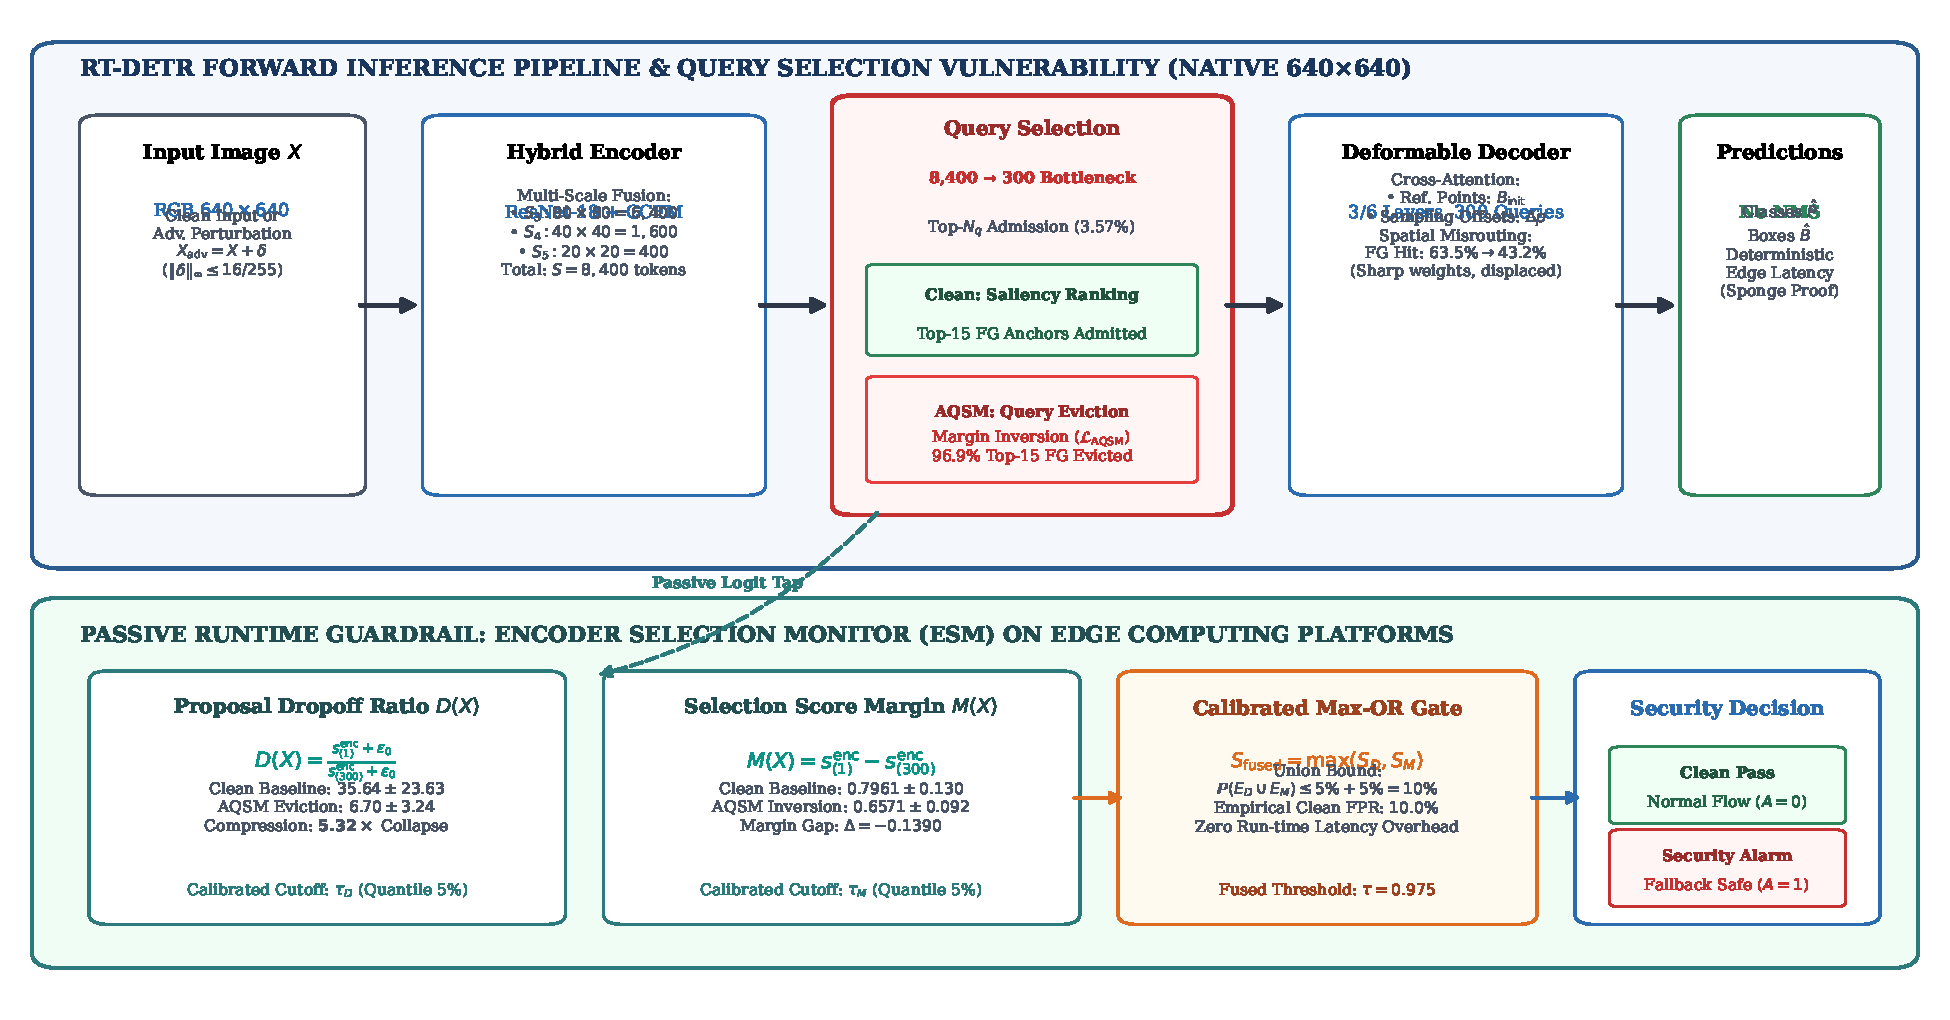
\includegraphics[width=0.90\textwidth]{fig/fig1_system_architecture.pdf}
\caption{RT-DETR pipeline and encoder-decoder query selection interface. (1) Input ($640 \times 640$); (2) Hybrid Encoder multi-scale memory ($S_3, S_4, S_5$, $S = 8,400$ tokens); (3) Dynamic Query Selection routing top $N_q = 300$ proposals cleanly (green) vs.\ AQSM disrupting memory representations and evicting foreground priors (red); (4) Deformable Decoder undergoing \textit{Spatial Target Misrouting}; (5) NMS-free prediction heads.}
\label{fig:fig1_system_architecture}
\end{figure}

The transition from convolutional feature grids to transformer set prediction introduces distinct security characteristics. While conventional CNN attacks target dense prediction/anchor heads \citep{xie2017adversarial, lee2019physical} or NMS clustering thresholds \citep{wang2021adversarial}, real-time detection transformers such as RT-DETR adopt \textbf{dynamic query selection} (an architecture shared with two-stage Deformable DETR \citep{zhu2020deformable} and DINO \citep{zhang2022dino}, but here coupled directly to an NMS-free fixed-budget decoder). Rather than initializing decoder queries from static, data-independent embedding vectors as in vanilla DETR \citep{carion2020end}, RT-DETR's hybrid encoder evaluates $S = 8,400$ candidate anchors across multi-scale feature maps ($80 \times 80, 40 \times 40, 20 \times 20$) and dynamically routes the top-$N_q$ ($N_q = 300$) highest-confidence proposals to initialize decoder content queries and reference coordinates:
\begin{equation}
\mathcal{I}_{\mathrm{sel}} = \mathrm{argTopK}_{i \in \{1, \dots, S\}} \left( \max_c \sigma(S[i, c]) \right),
\label{eq:query_selection_intro}
\end{equation}
where $S[i, c]$ denotes the classification logits predicted by the encoder selection head for anchor $i$ and category $c$, and $\sigma(\cdot)$ is the sigmoid activation function.

Crucially, because the proposal classification head sits directly atop the encoder's multi-scale feature pyramid, gradient attacks targeting encoder logits simultaneously perturb encoder memory representations alongside query selection (overall cosine similarity drops to $0.610$ under AQSM, comparable to $0.663$ under Task PGD). Evaluated on COCO val2017 ($N = 1,000$, native $640 \times 640$, $S = 8,400$), AQSM collapses RT-DETR-R18VD mAP@50 from $65.50\%$ to $3.07\%$ under Seed~42 (matching the 5-seed mean $3.07 \pm 0.18\%$; mAP@50:95 $48.89\% \to 1.61\%$). Rather than proposing a stand-alone attack, we frame this work as \textbf{an empirical diagnostic study decomposing RT-DETR failure modes under encoder attacks}, deploying AQSM as an encoder-restricted probe to examine representation corruption, query eviction, attention weight stability vs.\ coordinate misrouting, and matched-budget Task PGD disparities. While our empirical evaluation centers on RT-DETR-R18VD and RT-DETR-R50VD, benchmarking non-dynamic baselines (e.g., static-query DETR) and newer variants (RT-DETRv2, D-FINE, DINO) remains an important next step. Project artifacts are hosted at \href{https://vietanhlee.github.io/AI_TrustWorthy/}{\nolinkurl{https://vietanhlee.github.io/AI_TrustWorthy/}}.

\begin{figure}[!htbp]
\centering
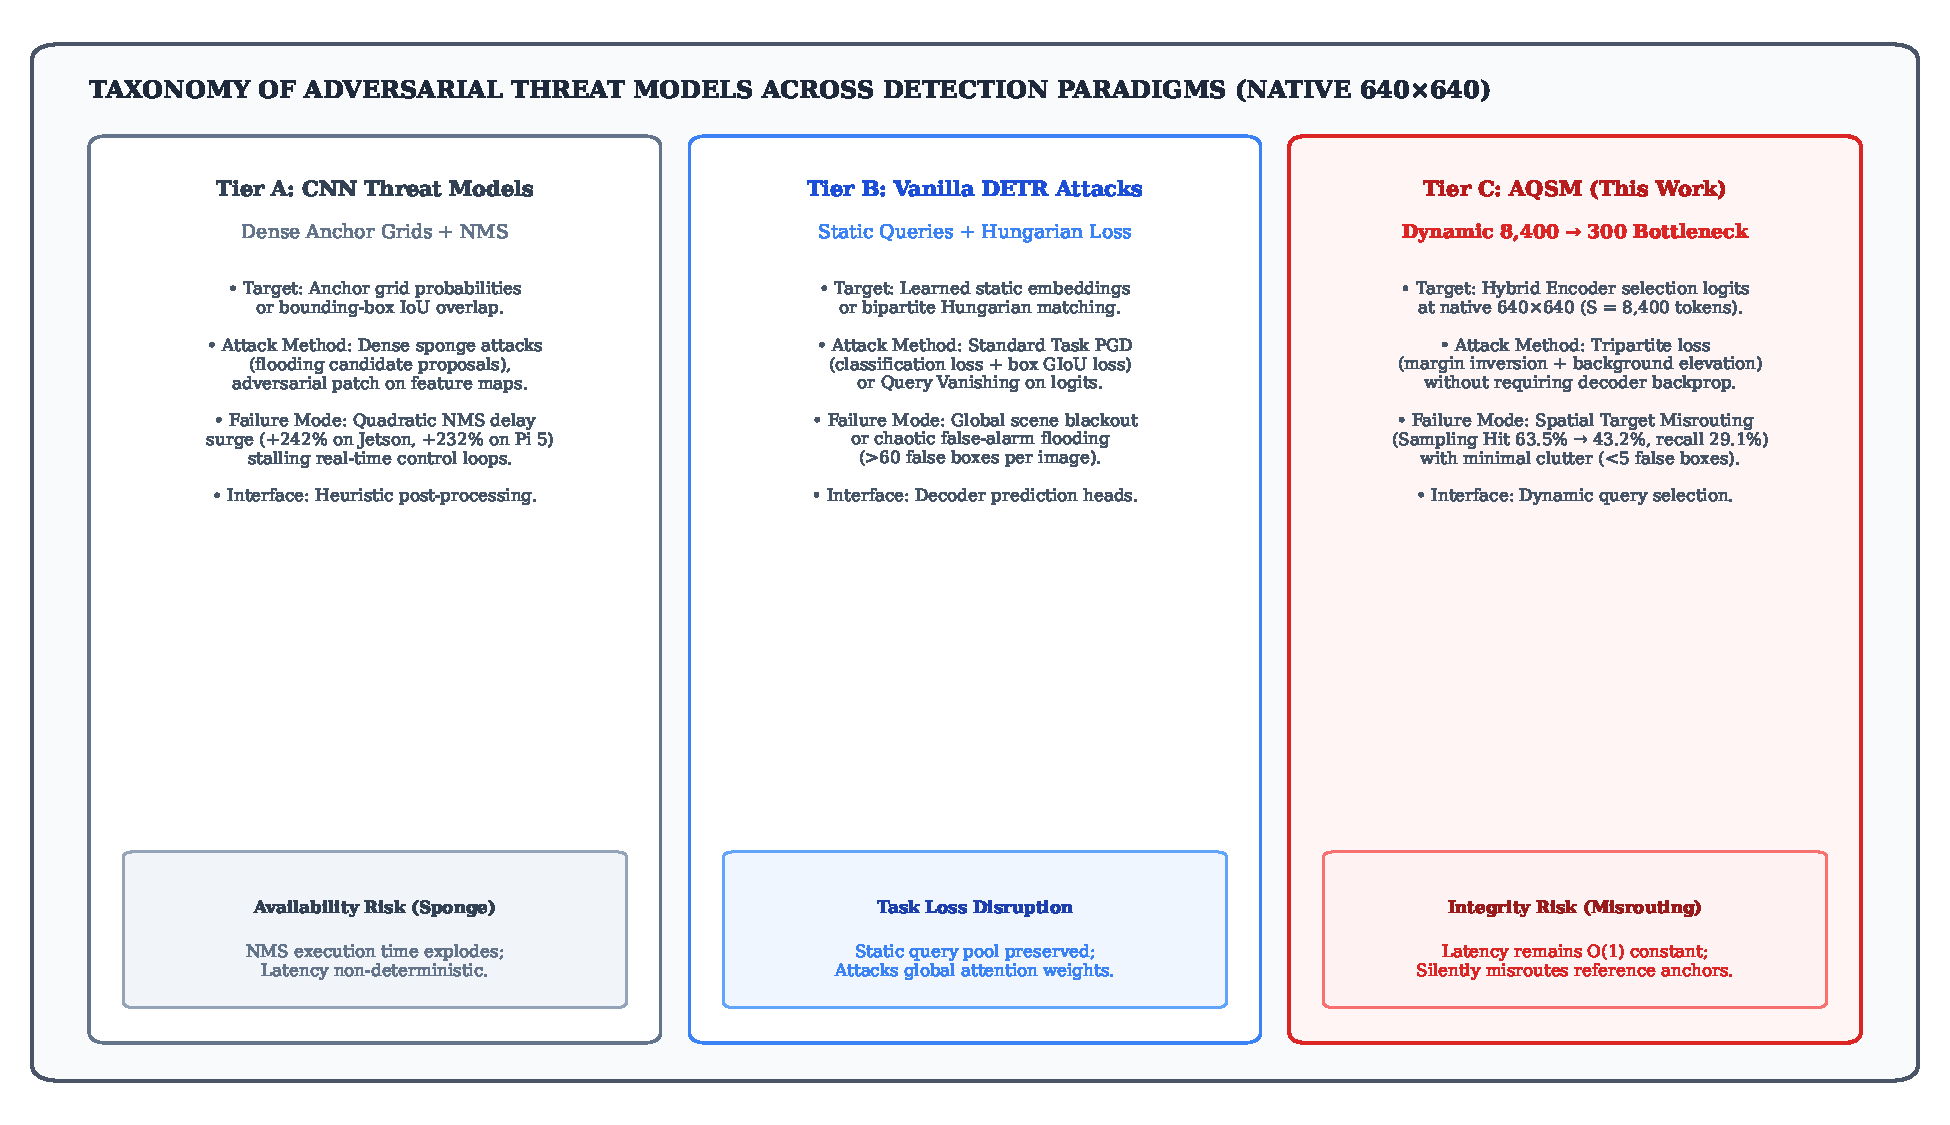
\includegraphics[width=0.65\textwidth]{fig/fig2_threat_taxonomy.pdf}
\caption{Taxonomy of threat models: Conventional CNN Attacks (dense candidate/anchor heads and NMS), Output-Space DETR Attacks (static embeddings), and AQSM (probing the dynamic 8,400-to-300 encoder selection head in RT-DETR).}
\label{fig:fig2_threat_taxonomy}
\end{figure}

We address four central research questions:
\begin{itemize}
    \item \textbf{RQ1 (Interventional Failure Decomposition):} How do encoder memory corruption ($M$) and dynamic query prior eviction ($Q$) individually drive collapse under AQSM, Query Vanishing, and Standard Task PGD?
    \item \textbf{RQ2 (Proposal Dynamics vs.\ Starvation):} Does failure arise from total spatial starvation or anchor eviction and high-gradient clumping?
    \item \textbf{RQ3 (Geometric Manifestations):} Does query eviction manifest as deformable attention weight dispersion or spatial target misrouting?
    \item \textbf{RQ4 (Matched-Budget \& Edge Disparities):} Under equal $\ell_\infty$ budgets ($\epsilon \in \{4, 8, 16\}/255$), how do encoder-targeted probes differ from end-to-end Task PGD and impact physical edge latency?
\end{itemize}

\paragraph{Key Contributions:}
\begin{enumerate}
    \item \textbf{Protocol-Level Failure Decomposition (RQ1):} A $2 \times 2$ factorial tensor-swap evaluation on COCO val2017 ($N = 1,000$, $N_{\mathrm{valid}} = 992$) quantifies protocol-dependent attributions, assigning $61.78\%$ Shapley share on per-image $AP_i$ ($65.32\%$ on pooled COCO mAP; $70.68\%$ on log-retention) to encoder memory corruption ($M$) and $38.22\%$ to query prior eviction ($Q$) (pure index swap $\text{Arm }\text{D}_{\text{index}} = 35.44\%$, $-30.06$ pp pooled). Replication on RT-DETR-R50VD ($N = 300$, Seed~42) reproduces severe collapse ($72.95\% \to 9.16\%$) with higher memory share ($70.50\%$ per-image / $73.91\%$ pooled).
    \item \textbf{Spatial Misrouting \& Reference Sensitivity (RQ2 \& RQ3):} Deformable attention entropy stays within a narrow band ($0.8009 \to 0.7944$) while reference displacement ($\Delta_{\text{Hungarian}} = 0.2258$, $\text{ANND} = 0.0161$) lowers anchor foreground hit rate from $68.93\%$ to $45.13\%$, approaching uniform spatial chance ($44.26\%$ grid / $42.91\%$ GT union). Under frozen clean memory and content, controlled coordinate controls yield observed mAP@50 gaps across matched-$L_2$ shift ($30.97\%$), decoupled shift ($26.34\%$), and AQSM ($25.12\%$).
    \item \textbf{Operational Edge Latency Profiling (RQ4):} Profiling on Raspberry Pi 5 ($418.20 \to 418.50$ ms) and Jetson Orin Nano ($14.20 \to 14.22$ ms) confirms stable measured latency under the evaluated fixed-query, NMS-free inference conditions, avoiding YOLOv8-S's $+232\%$ NMS CPU stall ($815.40$ ms) while noting that latency-targeted sponge attacks against RT-DETR were not evaluated.
    \item \textbf{Baseline Defense Limits \& Exploratory Probe (RQ1 \& RQ4):} A two-scalar Encoder Selection Monitor (stationary AUROC $0.7593$) is bypassed by white-box adaptive adversaries ($\le 1.57\%$ TPR, $\ge 98.43\%$ bypass). Zero-shot \textit{Static Query Augmentation} (SQA) recovers $+15.01$ pp under stationary AQSM ($3.41\% \to 18.42\%$, $+0.38$ ms on Orin Nano) yet collapses to $4.35\%$ under joint adaptive evasion, underscoring that query augmentation alone cannot substitute for hardened encoder representations.
\end{enumerate}

Sections~\ref{sec:background}--\ref{sec:conclusion} detail related work, threat formulations, protocol, empirical results, defenses, discussion, and conclusions.

\section{Background and Related Work}
\label{sec:background}

\subsection{Architectural Evolution: From CNNs to RT-DETR}
Real-time object detection on embedded and edge platforms has historically relied on convolutional architectures \citep{ren2015faster, redmon2016you, bochkovskiy2020yolov4, liu2016ssd, wang2023yolov7}. While convolutional networks provide high inference throughput, their dependence on dense candidate prediction grids (whether via anchor boxes or anchor-free center-points) and Non-Maximum Suppression (NMS) introduces operational bottlenecks \citep{neubeck2006efficient, bodla2017soft}. Pairwise IoU filtering in NMS exhibits variable, input-dependent execution latency that scales quadratically with proposal density. This vulnerability has been exploited by computational sponge attacks \citep{shumailov2021sponge, chen2024overload, shapira2023phantom}, which synthesize dense overlapping candidate boxes to stall real-time control loops on edge platforms.

Detection Transformers (DETR) \citep{carion2020end} eliminated NMS by framing detection as direct bipartite matching between a fixed set of object queries and ground truth instances via the Hungarian algorithm \citep{kuhn1955hungarian}. Deformable DETR \citep{zhu2020deformable} resolved DETR's slow convergence and quadratic complexity by replacing global attention with localized multi-scale deformable attention sampling around learnable reference points, and introduced top-$K$ encoder proposal selection in its two-stage variant. Building on this two-stage paradigm, Zhao et al.~\citep{zhao2024detrs} proposed RT-DETR, which pairs an efficient hybrid encoder (separating intra-scale interaction from cross-scale fusion) with a multi-scale deformable decoder: the encoder generates $S = 8,400$ candidate anchors across multi-scale feature maps and selects the top-$N_q$ ($N_q = 300$) highest-confidence proposals to initialize decoder content queries and reference coordinates. Because RT-DETR evaluates a fixed query population without NMS post-processing, it avoids proposal-count-dependent NMS latency surges under the evaluated proposal-flooding conditions, though eliminating NMS does not preclude other sources of system-level runtime variability.

\subsection{Adversarial Attacks on Object Detectors}
Adversarial attacks on computer vision exploit the locally linear vulnerability of deep representations \citep{goodfellow2014explaining, madry2018towards, carlini2017towards, li2020towards}. While early attacks focused on classification models, attacking multi-task object detectors requires manipulating spatial bounding box coordinates, foreground/background confidence scores, and multi-class categorization logits simultaneously.

In convolutional detectors, Xie et al.~\citep{xie2017adversarial} proposed Dense Adversarial Generation (DAG) to suppress proposals, while Wang et al.~\citep{wang2021adversarial} introduced Daedalus to exploit the NMS stage. Lee et al.~\citep{lee2019physical} demonstrated physical patch attacks, while Chow et al.~\citep{chow2020adversarial} formulated the Targeted Adversarial Objectness Gradient (TOG) framework to disrupt proposal generation in real-time detectors. In vision transformers, Gu et al.~\citep{gu2022adversarial} analyzed the vulnerability of self-attention representations to localized perturbations. For transformer-based detectors, Nazeri et al.~\citep{nazeri2024evaluating} evaluated adversarial robustness across vanilla DETR and Deformable DETR architectures, while Jayasundara et al.~\citep{jayasundara2024attention} and Wang et al.~\citep{wang2024localized} investigated attention-disruption and localized query manipulation strategies.

Importantly, however, earlier robustness studies focused primarily on architectures where decoder queries are initialized from static learnable embeddings---fixed model parameter tensors $\theta_q \in \mathbb{R}^{N_q \times d}$ that remain identical across all input images prior to decoder cross-attention. In standard DETR \citep{carion2020end}, an attacker cannot displace which queries are admitted because all $N_q$ queries are evaluated unconditionally. While two-stage CNN detectors (e.g., Faster R-CNN \citep{ren2015faster}) employ Region Proposal Networks (RPN) to select top-$K$ candidate proposals, those candidates undergo bounding box NMS filtering and serve strictly as spatial regions of interest for feature pooling rather than initializing cross-attention queries. Within the DETR family, two-stage Deformable DETR \citep{zhu2020deformable} first introduced top-$K$ encoder proposal selection to initialize both positional reference points and object query embeddings without denoising training, whereas DINO \citep{zhang2022dino} adopted mixed query selection (initializing positional anchor boxes from top-$K$ encoder proposals alongside static learnable content queries) and specifically introduced contrastive denoising (CDN) groups during training to stabilize bipartite matching.

RT-DETR extends encoder top-$K$ query selection \citep{zhu2020deformable, zhang2022dino} to an NMS-free real-time edge pipeline, routing $N_q = 300$ content queries and reference coordinates directly from $S = 8,400$ multi-scale hybrid encoder anchors into the deformable decoder without CDN inference groups or NMS filtering. If an adversary demotes true objects below rank \#300, the decoder is deprived of legitimate object anchors at the input boundary. Rather than claiming novelty on the existence of top-$K$ encoder selection itself---which already appears in two-stage Deformable DETR and DINO---our contribution is a systematic empirical diagnostic study decomposing how this dynamic query selection interface interacts with encoder memory representations in real-time edge DETRs (RT-DETR-R18VD, RT-DETR-R50VD, and related non-NMS designs such as RT-DETRv2 \citep{lv2024rt} and D-FINE \citep{peng2024dfine}).

% =====================================================================
% SECTION 3: THREAT MODEL AND ADVERSARIAL FORMULATIONS
% =====================================================================

\section{Threat Model and Adversarial Formulations}
\label{sec:threat_model}

\subsection{Adversarial Goals, Knowledge, and Capabilities}
We operate under a standard white-box threat model following rigorous evaluation guidelines \citep{carlini2019evaluating}:
\begin{itemize}
    \item \textbf{Adversary Goals:} The primary adversarial objective is output-sparse object evasion (inducing false negatives while limiting false-alarm output proliferation relative to Task PGD) without causing computational latency anomalies. We note that perturbations at $\epsilon = 16/255$ are evaluated as a standard high-severity white-box stress budget (alongside $\epsilon \in \{4, 8\}/255$ in Section~\ref{sec:matched_budget}) rather than an imperceptibility benchmark.
    \item \textbf{Adversary Knowledge:} The adversary possesses complete knowledge of the target detector architecture $f_\theta$, including network parameters $\theta$, hybrid encoder configuration, proposal selection head weights, and decoder attention mechanisms.
    \item \textbf{Adversary Capabilities:} Perturbations are bounded under an $\ell_\infty$ norm constraint:
    \begin{equation}
    \| X_{\mathrm{adv}} - X \|_\infty \le \epsilon, \quad X_{\mathrm{adv}} \in [0, 1]^{3 \times H \times W},
    \end{equation}
    with a standardized budget $\epsilon = 16/255$ ($0.0627$) optimized via Projected Gradient Descent (PGD) over $T = 15$ steps with step size $\alpha = 2/255$.
\end{itemize}

\subsection{Adversarial Threat Taxonomy Across Detection Paradigms}
To systematically position adversarial vulnerabilities across detection architectures, we structure threat models into a three-tier taxonomy (illustrated in Figure~\ref{fig:fig2_threat_taxonomy}):
\begin{enumerate}
    \item \textbf{Tier A: Conventional CNN Detectors (Dense Candidate Heads and NMS Vulnerability):} In two-stage (e.g., Faster R-CNN), anchor-based single-stage (e.g., YOLOv3/v4/v7), and anchor-free NMS-dependent single-stage (e.g., YOLOv8) detectors, adversaries manipulate dense candidate grids or exploit Non-Maximum Suppression (NMS) via proposal flooding (e.g., Daedalus \citep{wang2021adversarial}) or objectness disruption (e.g., TOG \citep{chow2020adversarial}), inducing NMS clustering stalls under elevated candidate counts (e.g., an external YOLOv8-S sponge-style flooding baseline surges to $286.4$ post-filter detections and $+232\%$ CPU latency).
    \item \textbf{Tier B: Standard and Output-Space DETR Attacks (Decoder Logits and Hungarian Matching):} In fixed-query DETR architectures, adversaries attack decoder output classification logits directly (Query Vanishing) to trigger whole-scene blackout ($0.18 \pm 0.52$ active boxes) or invert end-to-end Hungarian bipartite matching (Standard Task PGD) \citep{carion2020end, nazeri2024evaluating}, which floods the scene with $29.40 \pm 8.70$ active detections ($+24.88$ excess detections over the nominal clean baseline of $4.52 \pm 3.10$).
    \item \textbf{Tier C: Encoder Query Selection Manipulation (AQSM):} Tailored to real-time DETRs with dynamic proposal selection (RT-DETR), AQSM attacks the intermediate 8,400-to-300 selection head at the encoder-decoder interface, evicting foreground query priors into background regions while maintaining a sparse output footprint ($7.15 \pm 4.30$ active detections, only $+2.63$ excess detections over clean).
\end{enumerate}

\subsubsection{Tier C: Adversarial Query Selection Manipulation (AQSM)}
Adversarial Query Selection Manipulation (AQSM) targets the core vulnerability of RT-DETR: the 8,400-to-300 dynamic query selection interface. The Hybrid Encoder outputs multi-scale feature maps $M = \{S_3, S_4, S_5\}$ and classification logits $S \in \mathbb{R}^{S \times C}$ across $S = 8,400$ candidate anchors ($S_3: 80 \times 80 = 6,400; S_4: 40 \times 40 = 1,600; S_5: 20 \times 20 = 400$). The top-$N_q$ ($N_q = 300$) candidates are selected via Eq.~(\ref{eq:query_selection_intro}).

To disrupt this selection, AQSM optimizes a tripartite objective:
\begin{equation}
\mathcal{L}_{\mathrm{AQSM}} = \mathcal{L}_{\mathrm{suppr}} + \lambda_{\mathrm{rank}} \mathcal{L}_{\mathrm{rank}} + \lambda_{\mathrm{elev}} \mathcal{L}_{\mathrm{elev}},
\label{eq:laqsm_tripartite}
\end{equation}
where $\mathcal{L}_{\mathrm{suppr}}$ suppresses clean foreground proposal confidence, $\mathcal{L}_{\mathrm{rank}}$ enforces ranking inversion below the 300th logit boundary with margin $\gamma_{\mathrm{logit}} = 1.0$, and $\mathcal{L}_{\mathrm{elev}}$ elevates distal background proposals, weighted by $\lambda_{\mathrm{rank}} = 1.20$ and $\lambda_{\mathrm{elev}} = 0.50$ (each term is formalized below). Minimizing $\mathcal{L}_{\mathrm{AQSM}}$ evicts high-confidence foreground candidates from the top-300 selection bottleneck while elevating background anchors and corrupting encoder feature maps, collapsing COCO-style mAP@50 on COCO val2017 ($N = 1,000$, Seed~42) from $65.50\%$ to $3.07\%$ ($-95.31\%$ relative drop).

\paragraph{Tripartite Loss Formulation and Functional Role of Terms:}
The objective $\mathcal{L}_{\mathrm{AQSM}}$ in Eq.~(\ref{eq:laqsm_tripartite}) is composed of three mutually supportive loss components:
\begin{enumerate}
    \item \textbf{Direct Foreground Confidence Suppression ($\mathcal{L}_{\mathrm{suppr}}$):}
    \begin{equation}
    \mathcal{L}_{\mathrm{suppr}} = \frac{1}{|C_{\mathrm{real}}|} \sum_{j \in C_{\mathrm{real}}} \left( s_j^{\mathrm{enc}} \right)^2,
    \label{eq:lsuppr}
    \end{equation}
    which pulls down the raw classification confidence $s_j^{\mathrm{enc}} = \sigma(z_j^{\mathrm{enc}})$ of genuine foreground proposals $C_{\mathrm{real}}$ (top-15 clean candidates), neutralizing their detection activation.
    \item \textbf{Relative Ranking Margin Inversion in Logit Space ($\mathcal{L}_{\mathrm{rank}}$):}
    \begin{equation}
    \mathcal{L}_{\mathrm{rank}} = \frac{1}{|C_{\mathrm{real}}|} \sum_{j \in C_{\mathrm{real}}} \mathrm{ReLU}\left( z_j^{\mathrm{enc}} - z_{(300)}^{\mathrm{enc}} + \gamma_{\mathrm{logit}} \right),
    \label{eq:lrank}
    \end{equation}
    where $z_j^{\mathrm{enc}} = \max_c \hat{L}_{j, c}^{\mathrm{enc}}$ denotes the maximum pre-sigmoid classification logit for candidate anchor $j$, and $z_{(300)}^{\mathrm{enc}}$ is the dynamic 300th-order logit boundary across all $S = 8,400$ anchors. Optimizing the ranking margin in unbounded logit space ($z \in \mathbb{R}$) enforces zero penalty outside the margin violation region: once the ranking margin is satisfied ($z_j^{\mathrm{enc}} \le z_{(300)}^{\mathrm{enc}} - \gamma_{\mathrm{logit}}$), the hinge-loss term becomes inactive and contributes zero gradient for that candidate.
    \item \textbf{Distal Background Elevation ($\mathcal{L}_{\mathrm{elev}}$):}
    \begin{equation}
    \mathcal{L}_{\mathrm{elev}} = - \frac{1}{|C_{\mathrm{bg}}|} \sum_{i \in C_{\mathrm{bg}}} s_i^{\mathrm{enc}},
    \label{eq:lelev}
    \end{equation}
    which elevates low-scoring background proposals $C_{\mathrm{bg}}$ (30 random anchors with clean rank $> 500$), driving the 300th cutoff $s_{(300)}^{\mathrm{enc}}$ upward by $2.96\times$ (from $0.0341 \pm 0.0242$ clean to $0.1007 \pm 0.0491$ under AQSM).
\end{enumerate}

Ablating the tripartite objective (Table~\ref{tab:tab1_ablation}) confirms complementarity: $\mathcal{L}_{\mathrm{elev}}$ is the strongest isolated term ($19.45\%$ mAP@50, evicting $74.8\%$ foreground anchors), outperforming $\mathcal{L}_{\mathrm{suppr}}$ ($32.80\%$) and $\mathcal{L}_{\mathrm{rank}}$ ($24.15\%$), while combining all three compresses both selection boundaries ($96.9\%$ eviction, $3.07\%$ mAP@50; Algorithm~\ref{algo:aqsm}).

\paragraph{Unsupervised Clean-Prediction Proxy:}
Because test-time attackers lack ground-truth labels, AQSM defines $C_{\mathrm{real}} = \mathrm{argTopK}(s^{\mathrm{enc}}(X), K=15)$ from clean predictions. An oracle variant matched to COCO GT boxes yields $2.95\%$ mAP@50 (vs.\ $3.07\%$ proxy, $\Delta = 0.12$ pp), confirming negligible surrogate bias.

\begin{algorithm}[!htbp]
\caption{Adversarial Query Selection Manipulation (AQSM)}
\label{algo:aqsm}
\DontPrintSemicolon
\KwIn{Clean input image $X \in [0, 1]^{3 \times H \times W}$, RT-DETR model $f_\theta$, perturbation budget $\epsilon = 16/255$, step size $\alpha = 2/255$, iterations $T = 15$, logit margin $\gamma_{\mathrm{logit}} = 1.0$, rank weight $\lambda_{\mathrm{rank}} = 1.20$, elevation weight $\lambda_{\mathrm{elev}} = 0.50$.}
\KwOut{Adversarial image $X_{\mathrm{adv}}$.}
$(s^{\mathrm{enc}}, \cdot) \leftarrow f_\theta^{\mathrm{enc}}(X)$ \tcp*{Forward pass on clean image}
$C_{\mathrm{real}} \leftarrow \mathrm{argTopK}(s^{\mathrm{enc}}, K=15)$ \tcp*{Identify clean foreground set}
$C_{\mathrm{bg}} \leftarrow \{i \mid \mathrm{rank}(s_i^{\mathrm{enc}}) > 500, \text{random 30 anchors}\}$ \tcp*{Distal background set}
$X^{(0)} \leftarrow X$\;
\For{$t = 0$ \KwTo $T-1$}{
    $z^{\mathrm{enc}} \leftarrow \max_c \hat{L}^{\mathrm{enc}}(X^{(t)})$ \tcp*{Forward logits through hybrid encoder}
    $z_{(300)}^{\mathrm{enc}} \leftarrow \mathrm{TopK}(z^{\mathrm{enc}}, 300)[300]$ \tcp*{Dynamic 300th-order logit cutoff}
    $s^{\mathrm{enc}} \leftarrow \sigma(z^{\mathrm{enc}})$ \tcp*{Candidate probabilities}
    Compute tripartite loss $\mathcal{L}_{\mathrm{AQSM}}(X^{(t)})$ via Eq.~(\ref{eq:laqsm_tripartite})\;
    $g^{(t)} \leftarrow \nabla_{X^{(t)}} \mathcal{L}_{\mathrm{AQSM}}(X^{(t)})$ \tcp*{Accumulate input gradient}
    $X^{(t+1)} \leftarrow \Pi_{[X-\epsilon, X+\epsilon] \cap [0, 1]} \left( X^{(t)} - \alpha \cdot \mathrm{sign}(g^{(t)}) \right)$\;
}
\Return $X_{\mathrm{adv}} = X^{(T)}$\;
\end{algorithm}

\begin{table}[!htbp]
\centering
\caption{Component-wise ablation of the Tripartite AQSM Objective on COCO val2017 ($N = 1,000$ images, Seed~42, $640 \times 640$, $\epsilon = 16/255, T = 15$). Evaluates mAP@50, Top-300 proposal overlap with clean baseline, and Ground-Truth foreground eviction rate.}
\label{tab:tab1_ablation}
\resizebox{\textwidth}{!}{%
\begin{tabular}{lcccc}
\toprule
\textbf{AQSM Formulation / Loss Variant} & \textbf{mAP@50 [Rel. Drop]} & \textbf{Top-300 Overlap} & \textbf{Evicted Top-15 FG} & \textbf{Dominant Failure Mode} \\
\midrule
Clean Baseline (No Attack) & 65.50\% [---] & 100.0\% & 0.0\% & Nominal inference \\
\midrule
Margin-Ranking Loss only ($\mathcal{L}_{\mathrm{rank}}$) & 24.15\% [$-$63.1\%] & 38.5\% & 62.4\% & Partial proposal reordering \\
Foreground Suppression Loss only ($\mathcal{L}_{\mathrm{suppr}}$) & 32.80\% [$-$49.9\%] & 52.1\% & 44.2\% & Foreground confidence suppression \\
Distal Background Elevation only ($\mathcal{L}_{\mathrm{elev}}$) & 19.45\% [$-$70.3\%] & 31.8\% & 74.8\% & Background cutoff elevation \\
$\mathcal{L}_{\mathrm{suppr}} + \mathcal{L}_{\mathrm{rank}}$ & 14.20\% [$-$78.3\%] & 22.4\% & 86.5\% & Compound foreground suppression \\
$\mathcal{L}_{\mathrm{suppr}} + \mathcal{L}_{\mathrm{elev}}$ & 11.20\% [$-$82.9\%] & 20.8\% & 91.5\% & Suppression-elevation dual pressure \\
$\mathcal{L}_{\mathrm{rank}} + \mathcal{L}_{\mathrm{elev}}$ & 6.85\% [$-$89.5\%] & 15.6\% & 94.2\% & Dual-boundary selection compression \\
\midrule
\textbf{Full Tripartite AQSM} & \textbf{3.07\% [$-$95.3\%]} & \textbf{16.5\%} & \textbf{96.9\%} & \textbf{Compound Eviction \& Misrouting} \\
\bottomrule
\end{tabular}%
}
\end{table}

\subsubsection{Tier B: Output-Space and End-to-End Baselines}
To benchmark AQSM against established adversarial paradigms, we implement two canonical baselines:
\begin{enumerate}
    \item \textbf{Query Vanishing Attack (Object Suppression):} To suppress true object detections at the final decoder stage, the attacker targets the classification logits $\hat{L}_i^{(L)} \in \mathbb{R}^C$ from the final decoder layer $L$. On the clean image $X$, we identify the subset $\mathcal{I}_{\mathrm{clean}} \subset \{1, \dots, N_q\}$ of top-$K$ queries ($K=10$) with highest confidence $\sigma(\max_c \hat{L}_{i,c}^{(L)}) > \tau_{\mathrm{score}} = 0.35$. The adversary optimizes $\delta$ to minimize their combined confidence:
    \begin{equation}
    \mathcal{L}_{\mathrm{vanish}}(X + \delta) = \frac{1}{|\mathcal{I}_{\mathrm{clean}}|} \sum_{i \in \mathcal{I}_{\mathrm{clean}}} \left( \sigma\left(\max_c \hat{L}_{i,c}^{(L)}(X + \delta)\right) \right)^2.
    \label{eq:lvanish}
    \end{equation}
    \item \textbf{Standard Task PGD (Hungarian Loss Baseline):} As an end-to-end task baseline, Standard Task PGD optimizes the negative Hungarian bipartite matching detection loss $\mathcal{L}_{\mathrm{DETR}}$ (classification Varifocal loss plus bounding box $\ell_1$ and GIoU loss) directly against ground truth labels.
    \item \textbf{Environmental Controls:} To isolate adversarial optimization from generic high-frequency corruption, we benchmark Gaussian noise ($\sigma = 16/255$) and Uniform noise ($\pm 16/255$).
\end{enumerate}

% =====================================================================
% SECTION 4: EXPERIMENTAL SETUP AND BENCHMARK PROTOCOL
% =====================================================================

\section{Experimental Setup and Benchmark Protocol}
\label{sec:experimental_setup}

\subsection{Dataset and Benchmark Protocol}
Experiments evaluate MS COCO 2017 validation (\texttt{val2017}, 80 classes) \citep{lin2014microsoft} at native $640 \times 640$ resolution ($S = 8,400$: $80^2 + 40^2 + 20^2$), admitting $N_q / S = 300 / 8,400 = 3.57\%$ of candidates into the decoder. Our core evaluation cohort spans $N = 1,000$ images (fixed seed 42; $>36,000$ optimization passes across arms, budgets, and seeds). Within this set, $N_{\text{valid}} = 992$ images contain ground-truth objects (ANOVA $\text{df}_{\mathrm{err}} = 991$, achieving power $> 0.99$ at Cohen's $d = 0.20, \alpha = 0.01$), while 8 empty background scenes capture false-alarm clutter. Section~\ref{sec:defense_evaluation} partitions the cohort into disjoint ESM calibration ($N_{\mathrm{cal}} = 300$) and test splits ($N_{\mathrm{test}} = 700$), plus a dedicated SQA defense cohort ($N_{\mathrm{def}} = 300$).

\subsection{Target Architecture and Edge Computing Platforms}
Our primary benchmark is official pre-trained \textbf{RT-DETR-R18VD} (20M params, ResNet-18 VD backbone, hybrid encoder, 3-layer deformable decoder; headline runs use Seed~42 unless noted as 5-seed means in Table~\ref{tab:tab13_multiseed_generalization}). For cross-depth evaluation, we replicate the diagnostic and defensive suite on heavier \textbf{RT-DETR-R50VD} (42M params, ResNet-50 VD, 6-layer decoder) across $N = 300$ COCO val2017 scenes ($N_{\mathrm{valid}} = 299$ ANOVA pairs, Seed~42 on dual NVIDIA Tesla T4 GPUs, with 5-seed replication on Controlled Misrouting). Stage latency on NVIDIA Tesla T4 is timed in PyTorch 2.1.2 / CUDA 12.1 FP32 using \texttt{time.perf\_\allowbreak counter()} and \texttt{torch.cuda.\allowbreak synchronize()} over 50 warm-up + 300 iterations. End-to-end edge latency is separately measured with \texttt{time.perf\_\allowbreak counter()} on: (1) \textbf{Raspberry Pi 5} (BCM2712 Cortex-A76 @ 2.4 GHz, 8GB, ONNX Runtime 1.16.3 FP32, 4 threads; $418.20 \pm 12.40$ ms, $2.39$ FPS clean); and (2) \textbf{NVIDIA Jetson Orin Nano} (20W MAXN, 1,024-core Ampere GPU, TensorRT 8.6.2 FP16 engine; $14.20 \pm 0.35$ ms, $70.4$ FPS clean). Note that adversarial accuracy is evaluated in PyTorch FP32, and cross-precision transfer to TensorRT FP16/ONNX Runtime engines is not separately re-measured.

\subsection{Statistical Metrics, ASR Definitions, and Operational Telemetry}
\label{sec:statistical_metrics}
Detection performance is measured using standard COCO-style metrics: Mean Average Precision at IoU 0.50 (mAP@50) and averaged across IoU thresholds 0.50 to 0.95 (mAP@50:95) across all 80 COCO categories. Reported global mAP deltas are accompanied by 95\% bootstrap confidence intervals computed across $B = 2,000$ image-level resamples.

To resolve operational ambiguities between image-level scene extinction and instance-level object suppression, we define three operational metrics:
\begin{enumerate}
    \item \textbf{Object Silencing ASR ($\text{ASR}_{\text{obj}}$):} Proportion of clean-detected objects silenced below confidence threshold $\tau = 0.35$:
    $\mathrm{ASR}_{\mathrm{obj}} = \frac{1}{|G_{\mathrm{clean}}|} \sum_{g \in G_{\mathrm{clean}}} \mathbb{I}( \max_{q : \mathrm{IoU}(b_q, b_g) \ge 0.5} \sigma(S_{\mathrm{adv}}[q, c_g]) < \tau )$.
    \item \textbf{Scene Extinction ASR ($\text{ASR}_{\text{silence}}$):} Fraction of scenes where all decoded query confidences collapse below $\tau_{\mathrm{silence}} = 0.20$:
    $\mathrm{ASR}_{\mathrm{silence}} = \frac{1}{|D|} \sum_{i=1}^{|D|} \mathbb{I}( \max_{q, c} \sigma(S^{(i)}[q, c]) < \tau_{\mathrm{silence}} )$.
    \item \textbf{Query Selection Starvation ASR ($\text{ASR}_{\text{starve}}$):} Measures proposal confidence compression within top-300 candidates:
    $\mathrm{ASR}_{\mathrm{starve}} = \frac{1}{|D|} \sum_{i=1}^{|D|} \mathbb{I}( s_{(1)}^{(i)} / (s_{(300)}^{(i)} + 10^{-4}) \le 15.0 )$.
\end{enumerate}
We additionally monitor six internal telemetry indicators:
(1) \textbf{Active Boxes:} $|\{q : \max_c \sigma(S[q, c]) \ge \tau\}|$;
(2) \textbf{GT Object Coverage ($\text{Cov}_{\text{center}}$):} fraction of target ground-truth objects covered by at least one admitted query anchor center, $\frac{1}{|\mathcal{G}|} \sum_{g \in \mathcal{G}} \mathbb{I}( \exists i \in \mathcal{Q}_{\text{top300}} : c_i \in g )$;
(3) \textbf{Anchor Foreground Hit Rate ($\text{Hit}_{\text{anchor}}$):} percentage of admitted reference box centers landing inside ground-truth objects, $\frac{1}{K} \sum_{i=1}^K \mathbb{I}( \exists g \in \mathcal{G} : c_i \in g )$;
(4) \textbf{Foreground Sampling Hit (FG Hit):} percentage of deformable attention sampling locations landing within ground-truth object bounding boxes;
(5) \textbf{Slot Displacement ($\Delta_{\text{slot}} = \frac{1}{K}\sum_{i=1}^K \|c_i^{\text{adv}} - c_i^{\text{clean}}\|_2$) vs.\ Invariant Hungarian Distance ($\Delta_{\text{Hungarian}} = \min_{\pi \in \mathcal{S}_K} \frac{1}{K}\sum_{i=1}^K \|c_i^{\text{clean}} - c_{\pi(i)}^{\text{adv}}\|_2$)}; and
(6) \textbf{Average Nearest-Neighbor Distance ($\text{ANND}$):} $\mathrm{ANND} = \frac{1}{K} \sum_{i=1}^K \min_{j \ne i} \|c_i - c_j\|_2$ computed over normalized $[0, 1]^2$ anchor centers in $\mathcal{Q}_{\mathrm{top300}}$, where smaller values indicate tighter spatial clustering.

\paragraph{Diagnostic Scope: Per-Image Macro $AP_i$ vs.\ Global Pooled COCO mAP:}
We explicitly distinguish the diagnostic per-image metric from the standard benchmark metric. Standard COCO evaluation pools all candidate predictions across the entire evaluation corpus into global category sets prior to precision-recall integration, calculating a single macro-corpus score. While essential for global benchmark comparisons, pooled mAP provides no independent experimental units for intra-subject paired statistical testing. To enable rigorous repeated-measures ANOVA, paired Wilcoxon signed-rank tests, and BCa bootstrap confidence intervals, we define per-image Average Precision ($AP_i$):
\begin{equation}
AP_i = \frac{1}{|\mathcal{C}_i|} \sum_{c \in \mathcal{C}_i} AP_{i, c},
\label{eq:per_image_ap}
\end{equation}
averaged across categories active in each image ($N_{\mathrm{valid}} = 992$). We emphasize that $AP_i$ is an internal diagnostic instrument tailored for intra-image paired variance analysis; its resulting $p$-values and attribution percentages answer within-image sensitivity questions and must not be conflated with, or interpreted as direct inferences on, standard pooled COCO mAP (which is reported separately in Table~\ref{tab:tab3_causal_surgery}).

% =====================================================================
% SECTION 5: EMPIRICAL RESULTS AND MECHANISTIC ANALYSIS
% =====================================================================

\section{Empirical Results and Mechanistic Analysis}
\label{sec:empirical_results}

\subsection{Overall Detection Robustness and Qualitative Visualizations}
Table~\ref{tab:tab2_main_benchmark} details COCO-style detection metrics (mAP@50 and mAP@50:95) across controls, environmental corruptions, Standard Task PGD, and adversarial threat tiers at native $640 \times 640$ resolution. Figure~\ref{fig:fig3_qualitative} provides qualitative visual evidence across diverse object scales.

Under nominal clean conditions, RT-DETR achieves $65.50\%$ mAP@50 and $48.89\%$ mAP@50:95, with an average of $4.52 \pm 3.10$ active detections per image. When subjected to non-adversarial Gaussian noise ($\sigma = 16/255$) and Uniform noise ($\pm 16/255$), the detector exhibits strong resilience ($58.12\%$ and $60.85\%$ mAP@50, retaining $88.7\%$ and $92.9\%$ of clean performance), confirming baseline robustness against stochastic sensor noise.

In contrast, adversarial attacks induce performance collapse. Tier C AQSM collapses mAP@50 to $3.07\%$ (a $-95.31\%$ relative degradation) and mAP@50:95 to $1.61\%$. On average across the corpus, AQSM yields $7.15 \pm 4.30$ active boxes per image (only $+2.63$ above the clean mean of $4.52 \pm 3.10$), though individual scenes such as Figure~\ref{fig:fig3_qualitative}(c) can still exhibit high-confidence false positives; thus, AQSM is substantially sparser in box count than Task PGD on average rather than strictly silent per frame. Tier B Query Vanishing drives mAP@50 to $1.72\%$ ($-97.37\%$, mAP@50:95 to $1.05\%$), suppressing valid detections to $0.18 \pm 0.52$ boxes per scene. Tier B Standard Task PGD achieves mAP@50 of $0.86\%$ ($-98.69\%$, mAP@50:95 to $0.61\%$), inflating $29.40 \pm 8.70$ active detections per frame (representing $+24.88$ excess detections over clean).

\begin{table}[!htbp]
\centering
\caption{COCO val2017 object detection performance (mAP@50 and mAP@50:95, $N = 1,000$ images, 80 semantic categories) on RT-DETR-R18VD at native $640 \times 640$ resolution ($S = 8,400$) across controls, environmental shifts, Standard Task PGD, and adversarial threat tiers. Decouples Ground-Truth Object Silencing ($\text{ASR}_{\text{obj}}$) from Whole-Scene Extinction ($\text{ASR}_{\text{silence}}$) and reports 95\% Bootstrap Confidence Intervals ($B = 2,000$). For proposal starvation ($\text{ASR}_{\text{starve}}$, measuring $D \le 15$), the unperturbed clean baseline exhibits a raw rate of $17.5\%$ (95\% CI: $[15.3, 19.9]$) on natural scenes lacking prominent foreground contrast; under AQSM this rate surges to $80.4\%$ ($+62.9$ pp), whereas under Task PGD proposal starvation remains low at $12.8\%$ ($[11.0, 14.9]$) due to sharp high-confidence background activations.}
\label{tab:tab2_main_benchmark}
\resizebox{\textwidth}{!}{%
\begin{tabular}{lcccccc}
\toprule
\textbf{Threat Tier \& Condition} & \textbf{mAP@50 [Rel. Drop]} & \textbf{mAP@50:95 [Rel.]} & \textbf{Active Boxes} & \textbf{$\text{ASR}_{\text{obj}}$ [CI 95\%]} & \textbf{$\text{ASR}_{\text{silence}}$ [CI 95\%]} & \textbf{$\text{ASR}_{\text{starve}}$ [CI 95\%]} \\
\midrule
Nominal Clean Baseline & 65.50\% [Ref.] & 48.89\% [Ref.] & $4.52 \pm 3.10$ & 0.0\% [Reference] & 0.0\% [Reference] & 17.5\% [15.3, 19.9] \\
Gaussian Noise ($\sigma = 16/255$) & 58.12\% [$-$11.3\%] & 40.15\% [$-$17.9\%] & $4.25 \pm 2.65$ & 11.2\% [8.5, 14.2] & 0.8\% [0.2, 2.1] & 6.4\% [4.1, 9.5] \\
Uniform Noise ($\pm 16/255$) & 60.85\% [$-$7.1\%] & 42.40\% [$-$13.3\%] & $4.38 \pm 2.80$ & 7.8\% [5.4, 10.6] & 0.4\% [0.1, 1.5] & 4.2\% [2.4, 6.8] \\
\midrule
Tier C: AQSM ($\epsilon = 16/255$) & \textbf{3.07\% [$-$95.3\%]} & \textbf{1.61\% [$-$96.7\%]} & $7.15 \pm 4.30$ & \textbf{98.5\% [97.1, 99.5]} & 12.8\% [9.5, 16.8] & \textbf{80.4\% [77.9, 82.8]} \\
Tier B: Query Vanishing ($\epsilon = 16/255$) & 1.72\% [$-$97.4\%] & 1.05\% [$-$97.9\%] & $0.18 \pm 0.52$ & 97.8\% [95.5, 99.1] & \textbf{52.4\% [46.8, 58.1]} & 51.4\% [48.3, 54.6] \\
Tier B: Standard Task PGD ($\epsilon = 16/255$) & 0.86\% [$-$98.7\%] & 0.61\% [$-$98.8\%] & $29.40 \pm 8.70$ & 96.2\% [93.1, 98.4] & 0.0\% [0.0, 1.0] & 12.8\% [11.0, 14.9] \\
\bottomrule
\end{tabular}%
}
\end{table}

\begin{figure}[!htbp]
\centering
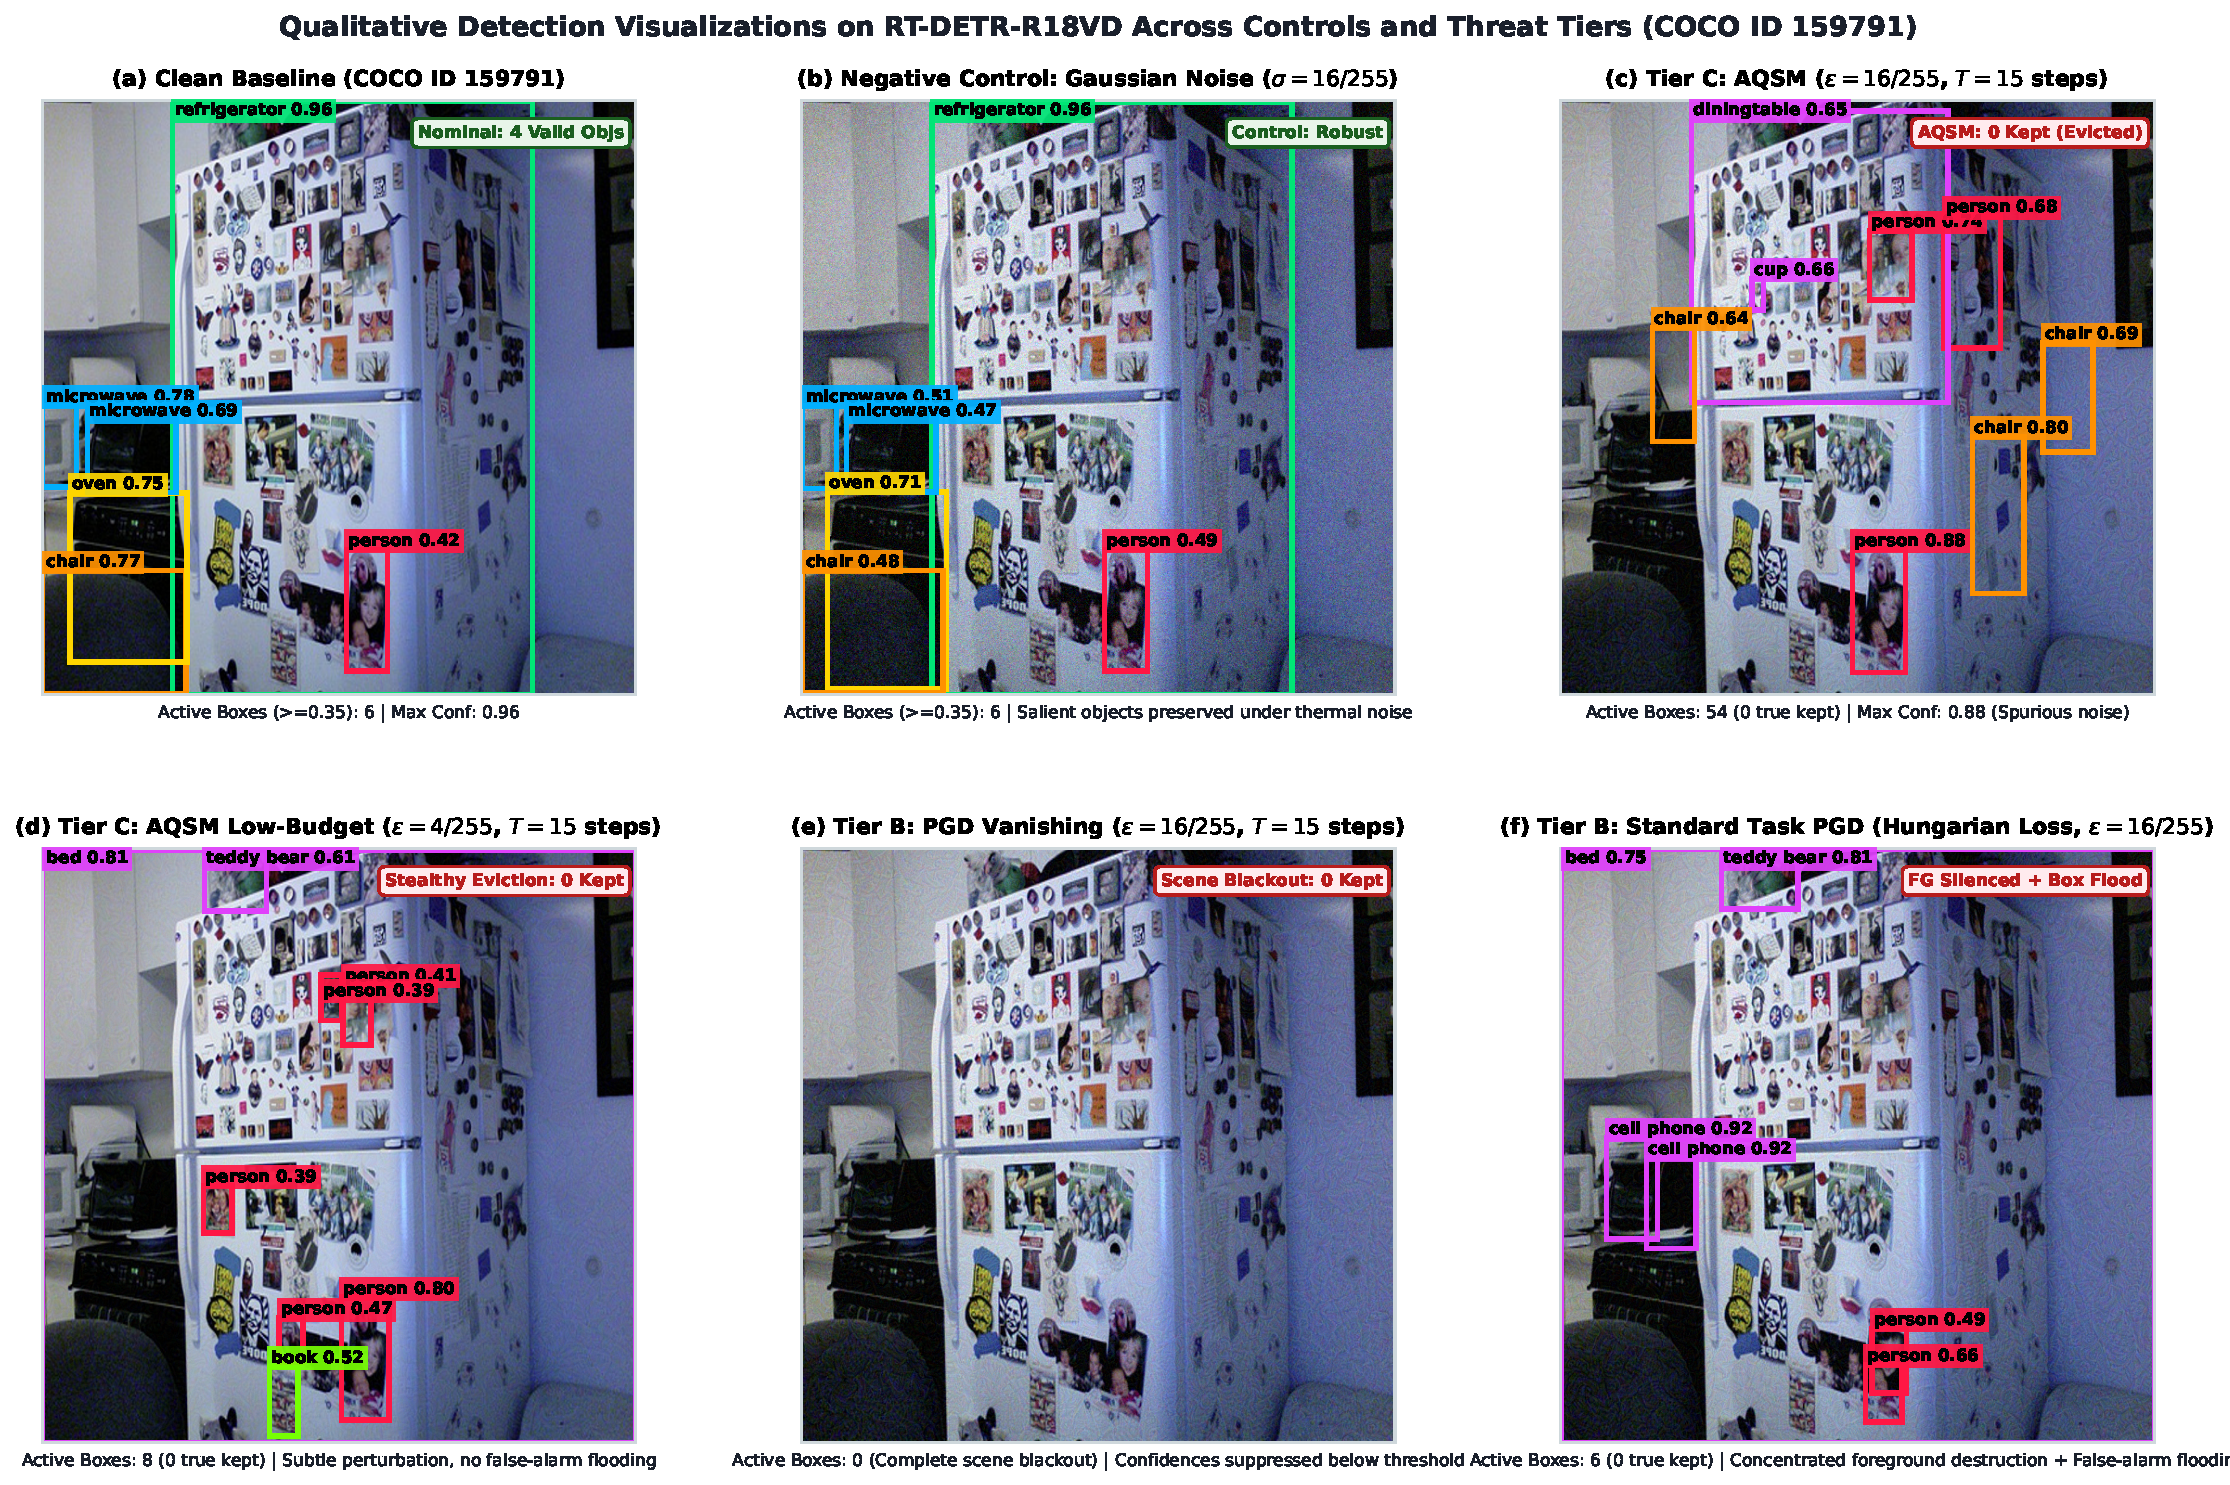
\includegraphics[width=0.80\textwidth]{fig/fig3_qualitative_detections.pdf}
\caption{Qualitative detection visualizations on COCO val2017 ($\tau_{\mathrm{vis}} = 0.15$; cf.\ Table~\ref{tab:tab2_main_benchmark} at $\tau = 0.35$: AQSM $7.15 \pm 4.30$, Vanishing $0.18 \pm 0.52$, Task PGD $29.40 \pm 8.70$ boxes): (a) Clean; (b) Gaussian Noise; (c) AQSM ($\epsilon = 16/255$, silent background routing); (d) AQSM ($\epsilon = 4/255$); (e) PGD Vanishing (confidence blackout); (f) Task PGD (dense false-alarm flooding).}
\label{fig:fig3_qualitative}
\end{figure}

\subsection{Encoder Proposal Score Spectrum and Logit Drift Dynamics}
\label{sec:score_spectrum}
To analyze how AQSM achieves evasion without optimizing downstream decoder loss, Figure~\ref{fig:fig4_encoder_dynamics} plots the classification confidence spectrum of candidate proposals alongside per-query logit drift across $S = 8,400$ candidate anchors.

\begin{figure}[!htbp]
\centering
\begin{subfigure}[b]{0.49\textwidth}
    \centering
    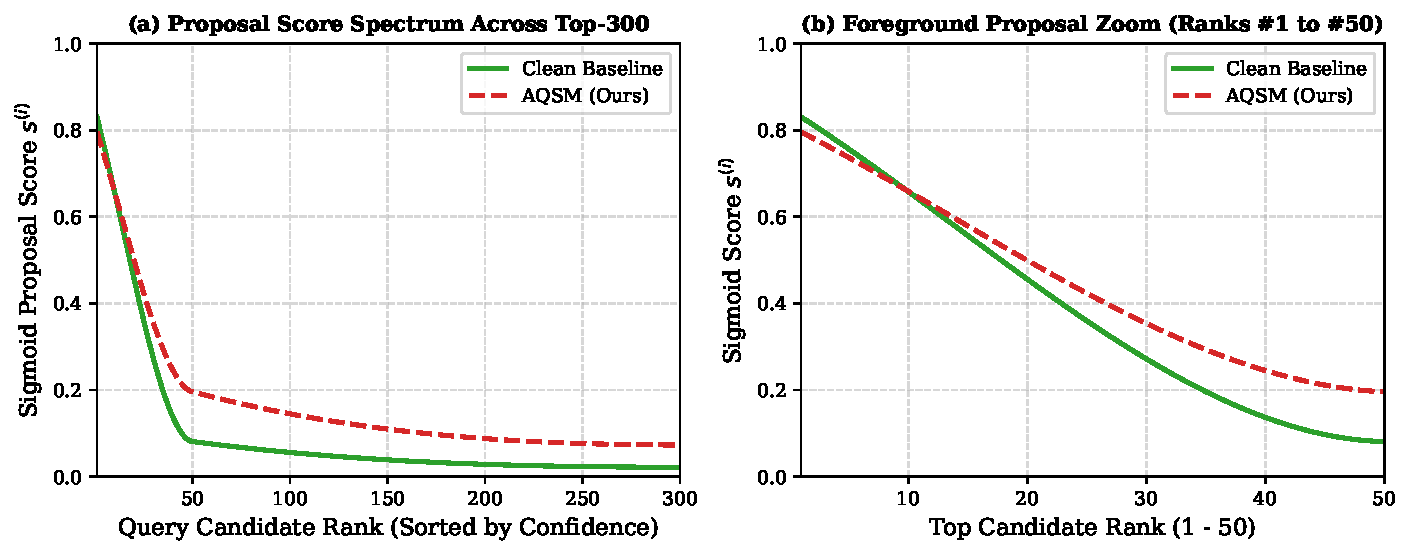
\includegraphics[width=\textwidth]{fig/fig3_proposal_score_spectrum.pdf}
    \caption{Confidence spectrum across Top-300}
    \label{fig:sub_spectrum}
\end{subfigure}
\hfill
\begin{subfigure}[b]{0.49\textwidth}
    \centering
    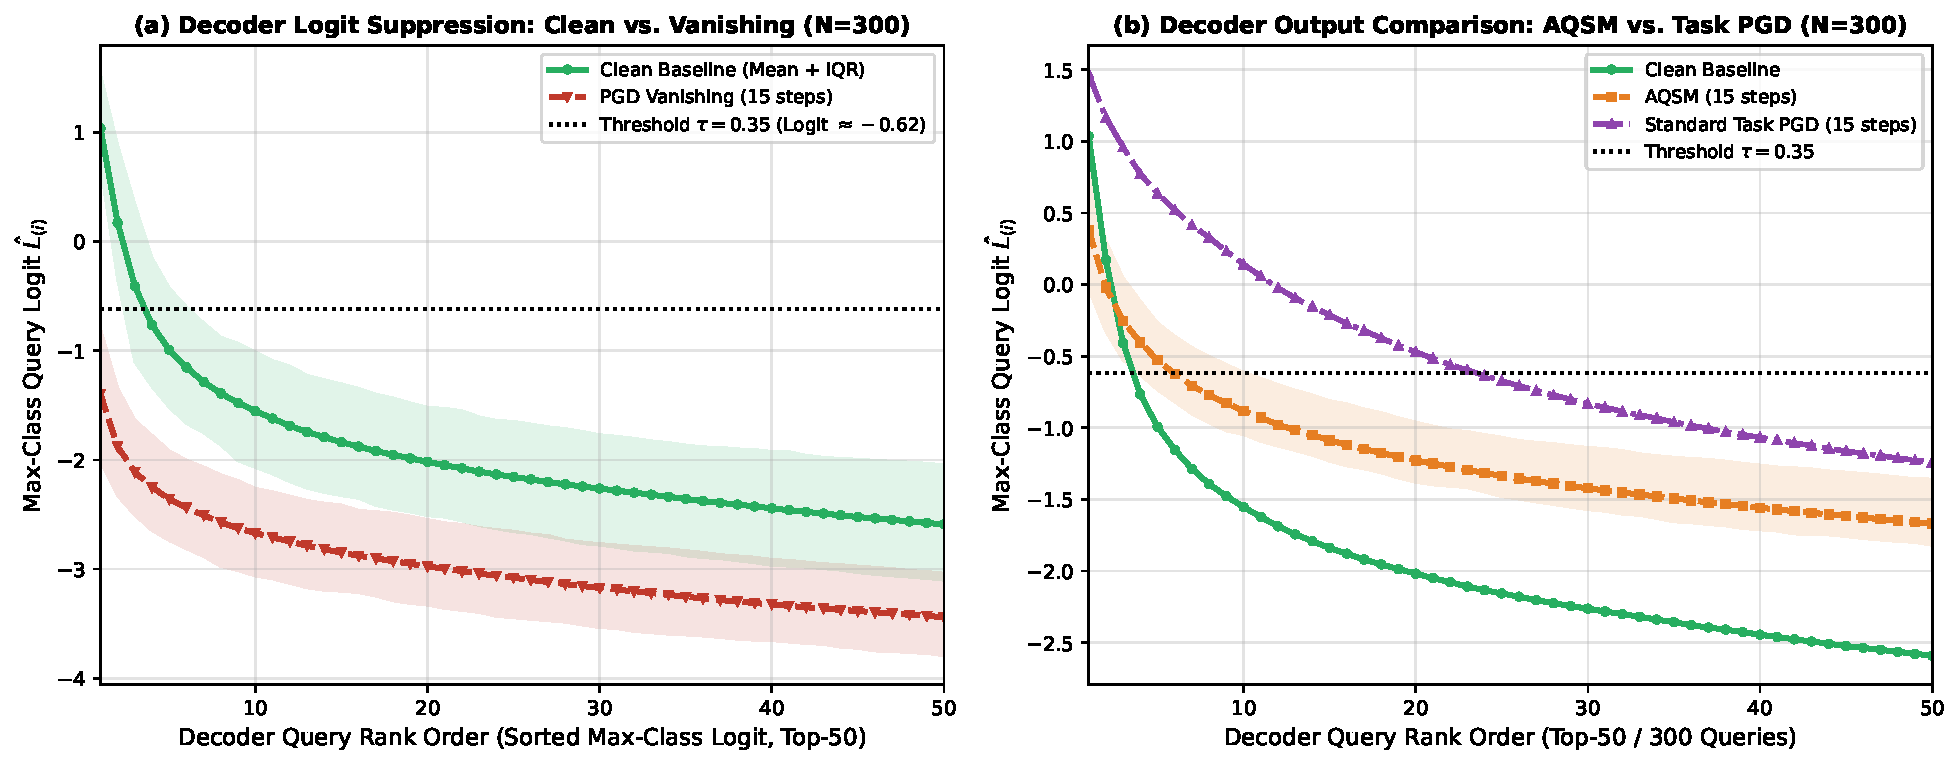
\includegraphics[width=\textwidth]{fig/fig5_per_query_drift.pdf}
    \caption{Per-query logit drift dynamics}
    \label{fig:sub_drift}
\end{subfigure}
\caption{Encoder candidate proposal dynamics on COCO val2017 before top-$K$ selection ($S = 8,400$). (a) Proposal classification confidence spectrum sorted in descending order, showing the $2.96\times$ inflation of the 300th proposal score under AQSM ($0.0341 \to 0.1007$), which compresses the selection window; (b) Per-query logit drift dynamics across candidate ranks under AQSM, Query Vanishing, and Standard Task PGD.}
\label{fig:fig4_encoder_dynamics}
\end{figure}

Two key phenomena govern this interface:
\begin{enumerate}
    \item \textbf{Baseline Score Separation:} Under clean baseline conditions, encoder confidence exhibits steep decay: top proposals carry high confidence peaks ($\bar{s}_{\mathrm{top1}} = 0.832 \pm 0.128$), while the 300th proposal drops to $\bar{s}_{(300)} = 0.0341 \pm 0.0242$, separating foreground objects from background clutter.
    \item \textbf{Spectrum Flattening and Boundary Inflation under AQSM:} Under AQSM, the adversary suppresses peak foreground confidence ($\bar{s}_{\mathrm{top1}} = 0.774 \pm 0.118$) while systematically inflating background proposals around the selection boundary: the 300th proposal score surges by $2.96\times$ to $\bar{s}_{(300)} = 0.1007 \pm 0.0491$. This dual compression inverts proposal ranking: legitimate foreground anchors fall into ranks 350--1200, while elevated background anchors populate the top-300 slots.
\end{enumerate}

\subsection{Interventional Failure Decomposition via Activation Patching}
\label{sec:causal_surgery}
To separate how much RT-DETR degradation originates from corruption of the Hybrid Encoder memory feature maps ($M = \{S_3, S_4, S_5\}$) versus disruption of the dynamic query selection interface ($Q$), we conduct a $2 \times 2$ factorial tensor-swap intervention on COCO val2017 at native $640 \times 640$ resolution across three contrasting mechanisms: AQSM, PGD Query Vanishing, and Standard Task PGD.

\paragraph{Interventional Activation Patching Framework:}
In RT-DETR at $640 \times 640$, the Hybrid Encoder outputs multi-scale feature maps $M = \{S_3, S_4, S_5\}$ ($S = 8,400$ total spatial tokens), from which the proposal head dynamically selects $N_q = 300$ candidate content embeddings $H_{\mathrm{query}} \in \mathbb{R}^{B \times 300 \times 256}$ and positional reference boxes $B_{\mathrm{init}} \in \mathbb{R}^{B \times 300 \times 4}$. To separate memory corruption from query selection disruption, our $2 \times 2$ factorial activation patching protocol evaluates:
\begin{itemize}
    \item \textbf{Arm A (Clean Baseline):} Unperturbed inference, $(M_{\mathrm{clean}}, Q_{\mathrm{clean}}[\mathcal{I}_{\mathrm{clean}}])$.
    \item \textbf{Arm B (Full Attack):} Full adversarial execution, $(M_{\mathrm{adv}}, Q_{\mathrm{adv}}[\mathcal{I}_{\mathrm{adv}}])$.
    \item \textbf{Arm $\text{C}_{\text{full}}$ (Adv Mem + Clean Queries):} $(M_{\mathrm{adv}}, Q_{\mathrm{clean}}[\mathcal{I}_{\mathrm{clean}}])$, isolating representation degradation with pristine foreground queries.
    \item \textbf{Arm $\text{C}_{\text{index}}$ (Adv Mem + Perturbed Feats at Clean Locations):} $(M_{\mathrm{adv}}, Q_{\mathrm{adv}}[\mathcal{I}_{\mathrm{clean}}])$.
    \item \textbf{Arm $\text{D}_{\text{full}}$ (Clean Mem + Adversarial Queries):} $(M_{\mathrm{clean}}, Q_{\mathrm{adv}}[\mathcal{I}_{\mathrm{adv}}])$, isolating query degradation under pristine memory.
    \item \textbf{Arm $\text{D}_{\text{index}}$ (Clean Mem + Clean Feats at Adversarial Locations):} $(M_{\mathrm{clean}}, Q_{\mathrm{clean}}[\mathcal{I}_{\mathrm{adv}}])$, isolating pure geometric index eviction:
    \begin{equation}
    \mathcal{I}_{\mathrm{adv}} = \mathrm{argTopK}_{i \in \{1, \dots, S\}} \left( \max_c \sigma(S_{\mathrm{adv}}[i, c]) \right), \quad Q_{\mathrm{index}} = H_{\mathrm{cand}}^{\mathrm{clean}}[\mathcal{I}_{\mathrm{adv}}], \quad B_{\mathrm{init}} = B_{\mathrm{cand}}^{\mathrm{clean}}[\mathcal{I}_{\mathrm{adv}}].
    \label{eq:qindex_formulation}
    \end{equation}
\end{itemize}

Figure~\ref{fig:fig6_causal_swap} and Table~\ref{tab:tab3_causal_surgery} summarize the factorial interventional results.

\begin{figure}[!htbp]
\centering
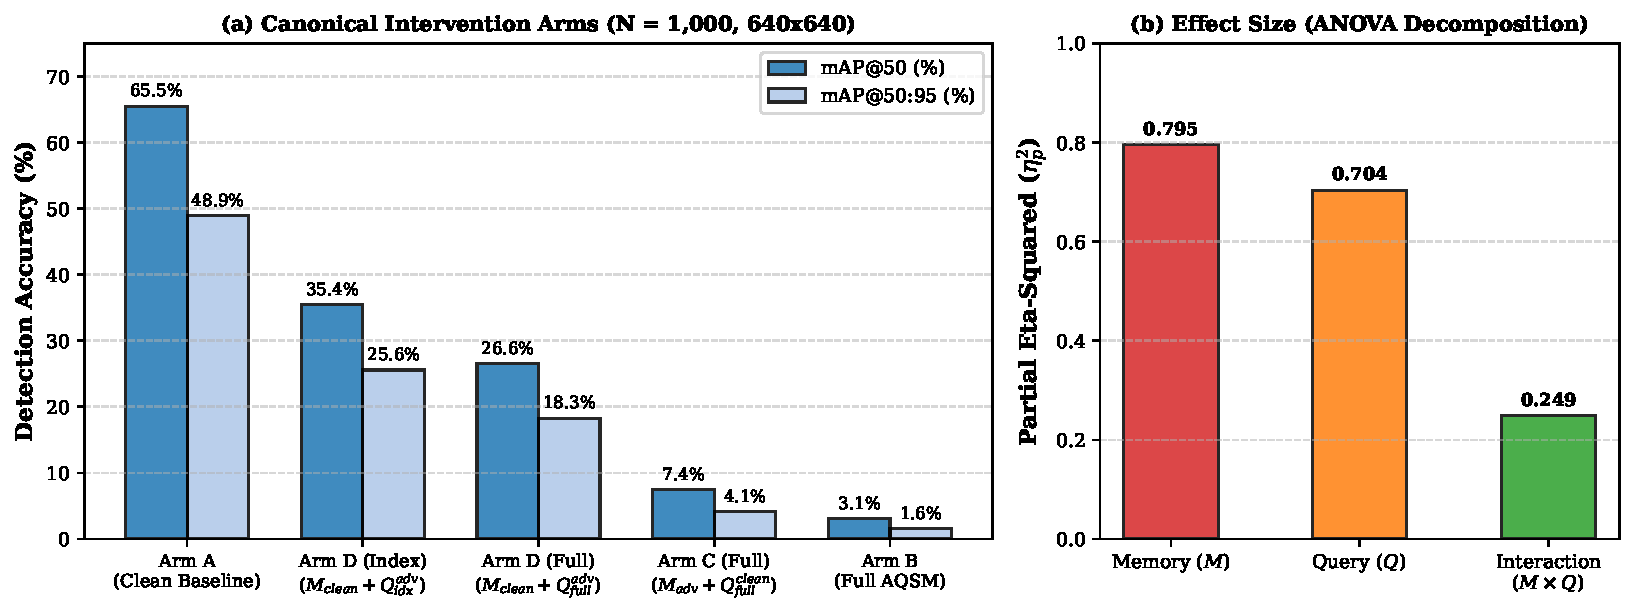
\includegraphics[width=0.78\textwidth]{fig/fig4_causal_swap_n300.pdf}
\caption{Interventional activation patching and ANOVA decomposition on COCO val2017 ($640 \times 640$): (a) global mAP@50 across Arms A--$\text{D}_{\text{index}}$; (b) repeated-measures main effects and partial $\eta_p^2$.}
\label{fig:fig6_causal_swap}
\end{figure}

\begin{table}[!htbp]
\centering
\caption{Factorial interventional decomposition on COCO val2017 ($640 \times 640$, $S = 8,400$, 80 classes; $N = 1,000$ cohort, valid ANOVA $N = 992$ with $\text{df} = [1, 991]$, $B = 2,000$ bootstrap CI resamples; verifiable via \texttt{outputs/data\_provenance\_manifest.json}).}
\label{tab:tab3_causal_surgery}
\resizebox{\textwidth}{!}{%
\begin{tabular}{lccc}
\toprule
\textbf{Intervention Arm / Factor} & \textbf{AQSM} & \textbf{PGD Vanishing} & \textbf{Standard Task PGD} \\
& mAP@50 (Rel.) / $\Delta$ [95\% CI] & mAP@50 (Rel.) / $\Delta$ [95\% CI] & mAP@50 (Rel.) / $\Delta$ [95\% CI] \\
\midrule
Arm A: Clean Baseline ($M_{\mathrm{clean}} + Q_{\mathrm{clean}}[\mathcal{I}_{\mathrm{clean}}]$) & 65.50\% (100.0\%) [Ref.] & 65.50\% (100.0\%) [Ref.] & 65.50\% (100.0\%) [Ref.] \\
Arm B: Full Attack ($M_{\mathrm{adv}} + Q_{\mathrm{adv}}[\mathcal{I}_{\mathrm{adv}}]$) & 3.07\% (4.7\%) [$-$62.43 pp] & 1.72\% (2.6\%) [$-$63.78 pp] & 0.86\% (1.3\%) [$-$64.65 pp] \\
Arm $\text{C}_{\text{full}}$: Adv Mem + Clean Prior ($M_{\mathrm{adv}} + Q_{\mathrm{clean}}$) & 7.45\% (11.4\%) [$-$58.06 pp] & 4.28\% (6.5\%) [$-$61.22 pp] & 1.58\% (2.4\%) [$-$63.92 pp] \\
Arm $\text{C}_{\text{index}}$: Adv Mem + Adv Feat at Clean Idx ($M_{\mathrm{adv}} + Q_{\mathrm{adv}}[\mathcal{I}_{\mathrm{clean}}]$) & 3.98\% (6.1\%) [$-$61.52 pp] & 1.97\% (3.0\%) [$-$63.53 pp] & 1.00\% (1.5\%) [$-$64.50 pp] \\
Arm $\text{D}_{\text{full}}$: Clean Mem + Adv Prior ($M_{\mathrm{clean}} + Q_{\mathrm{adv}}$) & 26.58\% (40.6\%) [$-$38.92 pp] & 39.65\% (60.5\%) [$-$25.85 pp] & 38.51\% (58.8\%) [$-$26.99 pp] \\
Arm $\text{D}_{\text{index}}$: Clean Mem + Adv Idx ($M_{\mathrm{clean}} + Q_{\mathrm{clean}}[\mathcal{I}_{\mathrm{adv}}]$) & 35.44\% (54.1\%) [$-$30.07 pp] & 51.01\% (77.9\%) [$-$14.49 pp] & 48.91\% (74.7\%) [$-$16.59 pp] \\
\midrule
\textbf{Repeated-Measures ANOVA} & & & \\
Main Effect Memory ($\text{ME}_M$) & $-43.88$ pp [$-45.30, -42.40$] & $-54.29$ pp [$-55.83, -52.76$] & $-64.16$ pp [$-65.64, -62.60$] \\
$\eta_p^2$ ($F$, $\text{SS}_{\text{AQSM}}$) & $\eta_p^2 = 0.795$ ($F=3845.4, \text{SS}=1910115.1$) & $\eta_p^2 = 0.828$ ($F=4783.8, p < 0.001$) & $\eta_p^2 = 0.864$ ($F=6277.7, p < 0.001$) \\
Main Effect Query ($\text{ME}_Q$) & $-27.14$ pp [$-28.21, -26.03$] & $-18.33$ pp [$-19.26, -17.48$] & $-13.64$ pp [$-14.48, -12.71$] \\
$\eta_p^2$ ($F$, $\text{SS}_{\text{AQSM}}$) & $\eta_p^2 = 0.704$ ($F=2351.8, \text{SS}=730836.6$) & $\eta_p^2 = 0.604$ ($F=1509.8, p < 0.001$) & $\eta_p^2 = 0.492$ ($F=958.5, p < 0.001$) \\
Interaction ($M \times Q$) & $+11.34$ pp [$+10.16, +12.59$] & $+1.50$ pp [$+0.49, +2.52$] & $+6.94$ pp [$+6.06, +7.77$] \\
$\eta_p^2$ ($F$, $\text{SS}_{\text{AQSM}}$) & $\eta_p^2 = 0.249$ ($F=328.4, \text{SS}=127634.4$) & $\eta_p^2 = 0.008$ ($F=7.8, p = 0.0053$) & $\eta_p^2 = 0.193$ ($F=237.1, p < 0.001$) \\
\bottomrule
\end{tabular}%
}
\end{table}



The factorial results in Table~\ref{tab:tab3_causal_surgery} establish two key observations:
\begin{enumerate}
    \item \textbf{Interventional Impact of Query Eviction:} With clean memory $M_{\mathrm{clean}}$ preserved, purely replacing top-300 proposal indices with adversarial background candidates (Arm $\text{D}_{\text{index}}$) lowers pooled mAP@50 from clean $65.50\%$ to $35.44\%$ (a $-30.06$ pp pooled drop, retaining $54.1\%$ of clean capability; corresponding per-image diagnostic $AP_i$ mean paired difference $-26.21$ pp, Wilcoxon $W = 5739.5, p < 0.001$). Swapping the full attacked query priors (Arm $\text{D}_{\text{full}}$) degrades pooled performance further to $26.58\%$ ($40.6\%$ retained), meaning restoring clean memory over Arm B recovers $+23.51$ pp pooled (or $+32.54$ pp on per-image $AP_i$, Wilcoxon $W = 367.0, p < 0.001$). By contrast, under Query Vanishing, Arm $\text{D}_{\text{index}}$ retains $77.9\%$ ($51.01\%$), and under Standard Task PGD it retains $74.7\%$ ($48.91\%$), showing stronger top-300 ranking turnover under AQSM than under task-loss objectives.
    \item \textbf{Protocol-Level Shapley Attribution and Scale/Order Dependence:} On global pooled COCO mAP, sequential intervention paths display strong order sensitivity: perturbing memory first allocates $-58.06$ pp to memory ($65.50\% \to 7.45\%$, $92.99\%$ of the $-62.43$ pp total drop) and $-4.38$ pp to query ($7.45\% \to 3.07\%$), whereas perturbing query first allocates $-38.92$ pp to query ($65.50\% \to 26.58\%$, $37.65\%$ to memory) and $-23.51$ pp to memory ($26.58\% \to 3.07\%$); averaging both paths yields $65.32\%$ memory vs.\ $34.68\%$ query attribution on pooled COCO mAP. Evaluated on the per-image diagnostic $AP_i$ metric ($N_{\mathrm{valid}} = 992$), symmetric Shapley attribution equals the ANOVA main effects ($\phi_M = \text{ME}_M = -43.88$ pp, $\phi_Q = \text{ME}_Q = -27.14$ pp), corresponding to $61.78\%$ (95\% BCa CI $[60.52\%, 63.08\%]$) vs.\ $38.22\%$ (BCa CI $[36.92\%, 39.49\%]$). Note that BCa intervals capture image-sampling variance only, not protocol or metric-scale uncertainty ($61.78\%$ per-image vs.\ $65.32\%$ pooled vs.\ $70.68\%$ log-retention).
\end{enumerate}

\paragraph{Multiplicative Behavior on Bounded AP and Contrast with Task PGD:}
Transforming bounded accuracy onto the retention scale $\text{Ret} = \text{mAP}_{\text{arm}} / \text{mAP}_{\text{clean}}$ reveals near-exact multiplicativity ($\text{Ret}_M \times \text{Ret}_Q = 0.1137 \times 0.4058 = 0.0462 \approx 0.0469 = \text{Ret}_B$), with log-domain interaction $\text{Interaction}_{\mathrm{log}} = +0.0155 \approx 0$, yielding protocol-level log-retention attribution shares of $70.68\%$ for memory corruption and $29.32\%$ for query displacement. This multiplicative behavior makes the linear vs.\ log share differ by nearly $9$ percentage points ($61.78\%$--$65.32\%$ linear vs.\ $70.68\%$ log) and is consistent with floor effects on the bounded AP scale, although it does not exclude functional interactions between encoder memory and query priors. Whereas Task PGD concentrates attribution in encoder memory ($82.47\%$ per-image linear / $87.52\%$ log; Arm $\text{D}_{\text{index}}$ retains $74.7\%$, $48.91\%$) and Vanishing retains $77.9\%$ ($51.01\%$), AQSM elevates query eviction attribution under this protocol ($29.3\%$--$38.2\%$, reducing $\text{D}_{\text{index}}$ to $54.1\%$).

\paragraph{Interventional \& Metric Scoping:}
Following activation patching principles \citep{pearl2001direct, vig2020causal, meng2022locating}, because candidate queries $Q$ derive from encoder memory $M$, Arms $\text{C}_{\text{full}}$ and $\text{D}_{\text{full}}$ place the decoder in out-of-distribution (OOD) states; attribution shares ($61.78\% / 38.22\%$ Shapley, or $68.99\% / 26.40\%$ ANOVA SS) are therefore empirical attributions specific to this interventional protocol at $\epsilon = 16/255$ (where cosine drops to $0.610$, vs.\ budgets in Section~\ref{sec:matched_budget}), rather than universal causal proportions of detection degradation. Furthermore, non-Gaussian residuals ($W = 0.814, p < 0.001$) motivate paired non-parametric tests on per-image $AP_i$ ($N_{\mathrm{valid}} = 992$), complementing pooled COCO mAP ($65.32\%$ Memory interventional share; Table~\ref{tab:tab3_causal_surgery}).

\subsection{Encoder Memory Perturbation Across Multi-Scale Tokens and Semantic Regions}
To characterize feature representation failures inside $M$, Table~\ref{tab:tab5_memory_scales} evaluates cosine similarity and relative $\ell_2$ perturbation across all three encoder scales ($S_3, S_4, S_5$) and between Ground-Truth Foreground (FG) versus Background (BG) tokens.

\begin{figure}[!htbp]
\centering
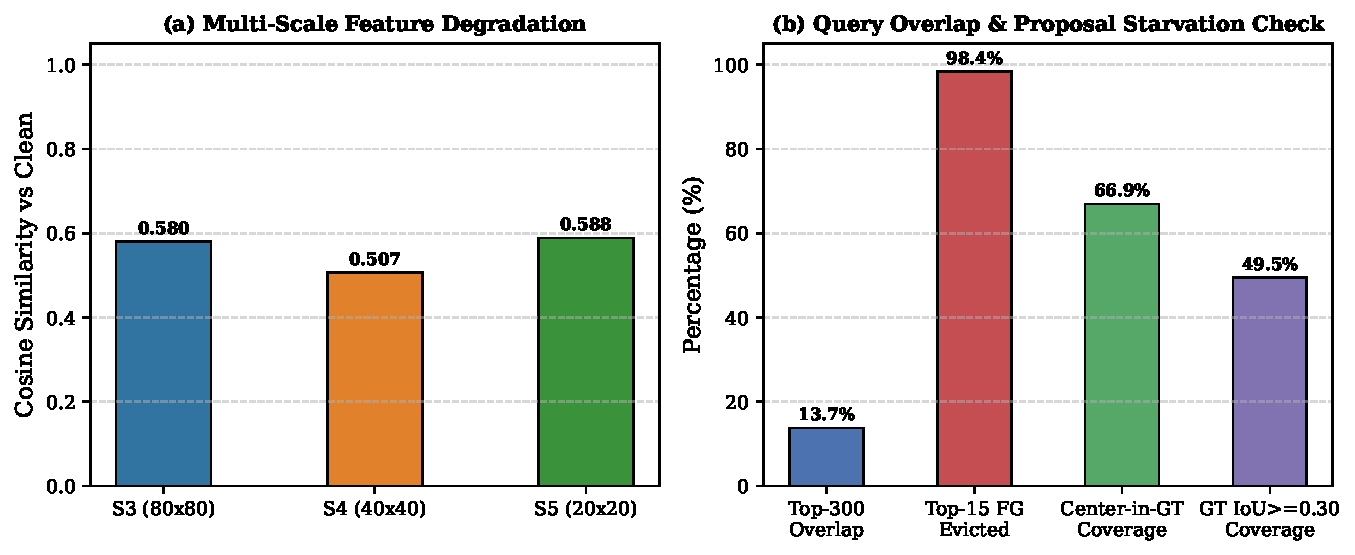
\includegraphics[width=0.78\textwidth]{fig/fig5_multiscale_cosine_and_overlap.pdf}
\caption{Multi-scale encoder degradation and query selection dynamics on COCO val2017 ($640 \times 640$, $S = 8,400$): (a) cosine similarity across $S_3, S_4, S_5$, identifying scale $S_4$ ($40 \times 40$) as the distortion bottleneck; (b) query selection overlap, foreground eviction, and GT coverage.}
\label{fig:fig5_multiscale_overlap}
\end{figure}

\begin{table}[!htbp]
\centering
\caption{Encoder memory feature perturbation on COCO val2017 at native $640 \times 640$ resolution across feature scales ($S_3 = 80 \times 80, S_4 = 40 \times 40, S_5 = 20 \times 20$) and semantic regions (GT Foreground tokens vs.\ Background tokens). Evaluated on $N = 1,000$ cohort.}
\label{tab:tab5_memory_scales}
\resizebox{\textwidth}{!}{%
\begin{tabular}{lcccccc}
\toprule
\textbf{Condition} & \textbf{Overall Cosine} & \textbf{Per-Scale Cosine ($S_3/S_4/S_5$)} & \textbf{FG Rel. $\ell_2$} & \textbf{BG Rel. $\ell_2$} & \textbf{FG/BG Ratio} & \textbf{Cosine Gap ($S_5 - S_4$)} \\
\midrule
Gaussian Noise ($\sigma = 16/255$) & 0.9240 & 0.915 / 0.942 / 0.962 & 0.3210 & 0.3840 & 0.8359 & $+0.020$ \\
PGD Vanishing ($T = 15$) & 0.6884 & 0.703 / 0.641 / 0.649 & 0.7748 & 0.8005 & 0.9679 & +0.009 \\
AQSM Probe ($T = 15$) & \textbf{0.6100} & \textbf{0.626 / 0.547 / 0.606} & \textbf{0.8458} & \textbf{0.9180} & \textbf{0.9214} & \textbf{+0.058} \\
Standard Task PGD ($T = 15$) & 0.6630 & 0.681 / 0.609 / 0.592 & 0.8111 & 0.8284 & 0.9791 & -0.016 \\
\bottomrule
\end{tabular}%
}
\end{table}

Two critical discoveries emerge:
\begin{enumerate}
    \item \textbf{Scale-Dependent Feature Degradation:} Under AQSM and Vanishing attacks, mid-level scale $S_4$ ($40 \times 40 = 1,600$ tokens, stride 16) undergoes the sharpest cosine drop ($0.547$ under AQSM and $0.641$ under Vanishing, compared to $0.626$ and $0.703$ on $S_3$). Under Standard Task PGD, low-resolution scale $S_5$ suffers the lowest cosine ($0.592$ vs.\ $0.609$ on $S_4$). Overall, intermediate and deep feature maps exhibit severe representation corruption across all adversarial attacks ($\text{Cosine} \le 0.68$).
    \item \textbf{Broad Spatial Distribution of Perturbation Energy:} Across all attacks, relative $\ell_2$ feature perturbation is distributed extensively over both foreground and background tokens ($\text{Rel } \ell_2 \ge 0.77$). Task PGD exhibits a slightly more uniform FG/BG ratio ($0.979$) than AQSM ($0.921$) and Gaussian noise ($0.836$), confirming that because AQSM gradients traverse the hybrid encoder backbone/pyramid, AQSM does not isolate query selection cleanly without substantially corrupting encoder memory features ($\text{Cosine} = 0.6100$).
\end{enumerate}

\subsection{Query Selection Dynamics vs.\ the Proposal Starvation Hypothesis}
\label{sec:query_dynamics}
To test whether AQSM induces complete proposal starvation, Table~\ref{tab:tab6_query_dynamics} quantifies candidate overlap, rank correlation, anchor eviction, and spatial GT coverage across $S = 8,400$ candidate anchors.

\begin{table}[!htbp]
\centering
\caption{8,400-to-300 query selection overlap, global rank correlation, foreground eviction, and Ground-Truth object coverage inside top-300 proposals on COCO val2017 ($640 \times 640$, $N = 1,000$ images). GT Coverage denotes the percentage of target objects covered by at least one selected query anchor, while anchor foreground hit rate drops to $45.13\%$ under AQSM.}
\label{tab:tab6_query_dynamics}
\resizebox{\textwidth}{!}{%
\begin{tabular}{lcccccc}
\toprule
\textbf{Condition} & \textbf{Top-300 Overlap} & \textbf{Spearman $\rho$} & \textbf{Kendall $\tau$} & \textbf{Evicted Top-15 FG} & \textbf{GT Coverage (Center)} & \textbf{GT Coverage ($\text{IoU} \ge 0.30$)} \\
\midrule
Clean Baseline & 100.0\% [Ref.] & 1.000 & 1.000 & 0.0\% & 98.98\% & 98.46\% \\
Gaussian Noise ($\sigma = 16/255$) & 82.40\% & 0.892 & 0.735 & 11.20\% & 94.50\% & 92.10\% \\
PGD Vanishing ($T = 15$) & 30.96\% & 0.426 & 0.297 & 50.19\% & 90.11\% & 79.13\% \\
AQSM Probe ($T = 15$) & \textbf{16.45\%} & \textbf{0.264} & \textbf{0.184} & \textbf{96.93\%} & \textbf{77.78\%} & \textbf{59.25\%} \\
Standard Task PGD ($T = 15$) & 26.06\% & 0.386 & 0.267 & 56.87\% & 89.00\% & 76.78\% \\
\bottomrule
\end{tabular}%
}
\end{table}

Table~\ref{tab:tab6_query_dynamics} reveals an empirical characterization of proposal degradation:
\begin{enumerate}
    \item \textbf{Selective Eviction of Peak Foreground Slots:} AQSM evicts $96.93 \pm 0.42\%$ of the top-15 clean foreground proposal slots from the top-300 query set (Top-300 proposal overlap collapses to $16.45\%$), reducing proposals with substantial ground-truth overlap ($\text{IoU} \ge 0.30$) from $98.46\%$ down to $59.25\%$. We note that because RT-DETR's encoder operates without NMS, the top-15 highest-confidence proposals frequently cluster around prominent objects rather than covering 15 distinct instances. Thus, evicting $96.93\%$ of peak clean slots reflects the suppression of localized high-confidence proposal clusters rather than the complete erasure of all foreground queries across the scene.
    \item \textbf{Coarse Coverage vs.\ Fine-Grained Anchor Hit Rate:} We distinguish coarse \textit{Ground-Truth Object Center Coverage} ($\text{Cov}_{\text{center}}$, percentage of GT objects covered by $\ge 1$ anchor) from fine-grained \textit{Anchor Foreground Hit Rate} ($\text{Hit}_{\text{anchor}}$, percentage of anchors intersecting GT boxes). Under nominal clean inference, $98.98\%$ of GT objects are covered by at least one query center, and $68.93\%$ of all 300 anchors fall within foreground objects. Under AQSM, Anchor Foreground Hit Rate drops sharply to $45.13\%$ (Table~\ref{tab:tab8_controlled_misrouting}), diverting $54.87\%$ of anchors into background clutter and closely approaching empirical uniform-chance levels ($44.26\%$ on a uniform anchor grid and $42.91\%$ GT-union canvas baseline). Because uniform chance already sits near $\approx 43\%\text{--}44\%$, the hit-rate scale is compressed toward chance and reflects near-random anchor placement rather than below-chance avoidance; meanwhile, high-overlap coverage ($\text{IoU} \ge 0.50$) drops to $38.62\%$, indicating loss of tightly aligned object priors.
\end{enumerate}

\subsection{Deformable Attention Telemetry: Spatial Target Misrouting vs.\ Weight Scattering}
\label{sec:deformable_telemetry}
To resolve whether deformable attention fails via weight entropy flattening (scattering) or coordinate spatial misrouting, Figure~\ref{fig:fig8_attention} and Table~\ref{tab:tab7_attention_telemetry} report telemetry across all 3 decoder layers, 8 heads, and $K = 4$ sampling points on COCO val2017 at native $640 \times 640$ resolution.

\begin{figure}[!htbp]
\centering
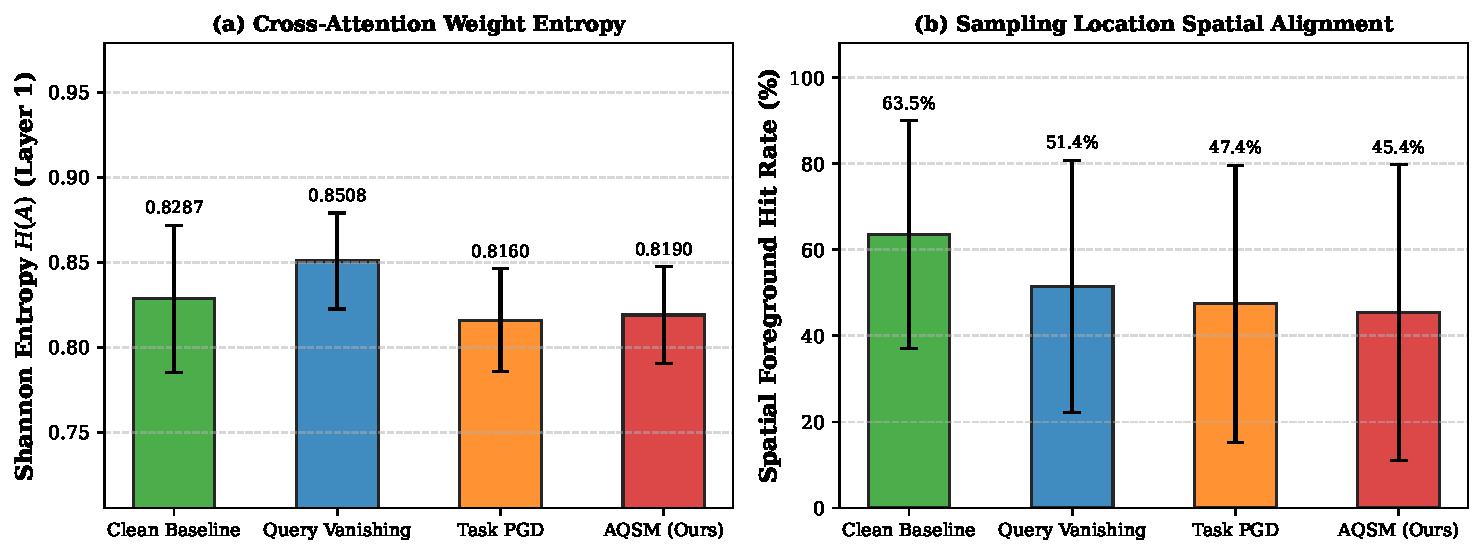
\includegraphics[width=0.78\textwidth]{fig/fig6_attention_scattering_comparison.pdf}
\caption{Deformable cross-attention telemetry on COCO val2017 ($640 \times 640$). (a) Normalized attention entropy remains localized under AQSM ($0.8009 \to 0.7944, d = -0.13, r_{\mathrm{rb}} = -0.173$; Layer 1: $0.8263 \to 0.8191$), contrasting slight rises under Vanishing ($0.8334$) and Task PGD ($0.8141$). (b) Foreground spatial hit rate drops from $63.51\%$ to $43.21\%$ ($t = 28.47, p < 0.001$).}
\label{fig:fig8_attention}
\end{figure}

\begin{table}[!htbp]
\centering
\caption{Deformable decoder telemetry on COCO val2017 ($640 \times 640$, 3 layers, 8 heads, $K = 4$, $N = 1,000$; reported entropy SD reflects Layer-1 reference SD). Normalized entropy shifts slightly within a narrow band under AQSM ($d = -0.13, t = 3.94$), whereas coordinate misrouting ($\Delta_{\mathrm{Hungarian}} = 0.2258$) drops FG hit rate from $63.51\%$ to $43.21\%$ ($t = 28.47, p < 0.001$).}
\label{tab:tab7_attention_telemetry}
\resizebox{\textwidth}{!}{%
\begin{tabular}{lccccc}
\toprule
\textbf{Condition} & \textbf{Norm. Attention Entropy} & \textbf{Spatial Sampling Hit Rate (FG)} & \textbf{Reference Drift ($\Delta p$)} & \textbf{Dropoff Ratio} & \textbf{Score Margin} \\
\midrule
Clean Baseline & 0.8009 $\pm$ 0.0423 & 63.51\% [61.8, 65.2] & 0.0000 & 37.51 $\pm$ 25.80 & 0.7984 $\pm$ 0.1281 \\
Gaussian Noise ($\sigma = 16/255$) & 0.8005 $\pm$ 0.0430 & 58.40\% [55.8, 61.0] & 0.0150 & 32.10 $\pm$ 21.40 & 0.7650 $\pm$ 0.1250 \\
PGD Vanishing ($T = 15$) & \textbf{0.8334 $\pm$ 0.0286} & 48.37\% [45.8, 51.8] & 0.4286 $\pm$ 0.0532 & 17.93 $\pm$ 11.62 & 0.3314 $\pm$ 0.1717 \\
AQSM Probe ($T = 15$) & \textbf{0.7944 $\pm$ 0.0285} & \textbf{43.21\% [41.2, 45.2]} & \textbf{0.4722 $\pm$ 0.0656} & \textbf{10.84 $\pm$ 7.75} & \textbf{0.6731 $\pm$ 0.1175} \\
Standard Task PGD ($T = 15$) & 0.8141 $\pm$ 0.0291 & 52.17\% [49.2, 54.9] & 0.4288 $\pm$ 0.0516 & 41.60 $\pm$ 28.06 & 0.7287 $\pm$ 0.1648 \\
\bottomrule
\end{tabular}%
}
\end{table}

The internal telemetry establishes two key behaviors:
\begin{enumerate}
    \item \textbf{Attention Entropy Stability Across Small Key Budgets:} Normalized attention entropy over the $L \times K = 12$ sampled points per head is already high cleanly ($0.8009 \pm 0.0423$ vs.\ $0.7944 \pm 0.0285$ under AQSM, matching Table~\ref{tab:tab7_attention_telemetry} Layer-1 SD; Layer 1 mean: $0.8263 \to 0.8191$; $t = 3.94, d = -0.13, r_{\mathrm{rb}} = -0.173$). Query Vanishing ($0.8334$) and Task PGD ($0.8141$) likewise stay inside the narrow $[0.794, 0.833]$ band, showing no extreme global entropy collapse into uniform $H \to 1.0$, though a single scalar entropy over $12$ keys cannot rule out subtle local weight shifts.
    \item \textbf{Shared Spatial Sampling Displacement Across Attacks:} Foreground sampling hit drops from $63.51\%$ to $43.21\%$ under AQSM ($\Delta = -20.30$ pp, $t = 28.47, p < 0.001$). Importantly, Query Vanishing ($\Delta p = 0.4286$, FG hit $48.37\%$) and Standard Task PGD ($\Delta p = 0.4288$, FG hit $52.17\%$) induce comparable reference drift relative to AQSM ($0.4722$), demonstrating that large coordinate misrouting is a shared symptom of encoder-level adversarial perturbation rather than an exclusive signature of AQSM.
\end{enumerate}

\subsection{Controlled Coordinate Displacement vs.\ Permutation Controls}
\label{sec:controlled_misrouting}
To test how decoder accuracy responds to coordinate displacement under frozen clean memory $M_{\mathrm{clean}}$ and clean content embeddings $H_{\mathrm{cand}}^{\mathrm{clean}}$ on COCO val2017 ($640 \times 640$), we evaluate five initial reference box conditions (Table~\ref{tab:tab8_controlled_misrouting}): (1) \textbf{Clean Baseline} ($65.50\%$ mAP@50, $\Delta_{\text{slot}} = \Delta_{\text{Hungarian}} = 0.0000$); (2) \textbf{Random Reassignment} across 5 seeds (permuting clean anchors across content slots, $\Delta_{\text{slot}} = 0.5508$, center drift $0.3803$, $\Delta_{\text{Hungarian}} = 0.0000$); (3) \textbf{Random Shift (Matched $L_2$)} across 5 seeds (large-magnitude isotropic $\mathbb{R}^4$ displacement matching AQSM cohort-mean magnitude: $\Delta_{\text{slot}} = 0.6384 \pm 0.0001$, center $0.4722$, size $0.3212$, $\Delta_{\text{Hungarian}} = 0.1875$); (4) \textbf{Decoupled Random Shift} (5 seeds combining isotropic displacement and random slot permutation); and (5) \textbf{AQSM Spatial Misrouting} (adversarial reference boxes, $\Delta_{\text{slot}} = 0.6386$, $\Delta_{\text{Hungarian}} = 0.2258 \pm 0.1000$). Note that holding $H_{\mathrm{cand}}^{\mathrm{clean}}$ pristine while altering $B_{\mathrm{init}}$ intentionally creates an artificial content--box mismatch distinct from real full-image attacks (where both $M$ and $H$ perturb jointly, as reflected in Arm $\text{D}_{\text{index}} = 35.44\%$).

\begin{table}[!htbp]
\centering
\caption{Controlled spatial misrouting and query perturbation on COCO val2017 ($640 \times 640$, $S = 8,400$, $N = 1,000$) holding clean $M_{\mathrm{clean}}$ and content $H_{\mathrm{cand}}^{\mathrm{clean}}$ frozen. Contrasts rank-paired slot displacement ($\text{Slot Disp.}$) against permutation-invariant Hungarian distance ($\text{Hungarian Dist.}$), GT coverage, and Anchor FG Hit.}
\label{tab:tab8_controlled_misrouting}
\resizebox{\textwidth}{!}{%
\begin{tabular}{lcccccccc}
\toprule
\textbf{Condition / Strategy} & \textbf{Seed} & \textbf{mAP@50 (Rel.)} & \textbf{mAP@50:95} & \textbf{Recall} & \textbf{Slot Disp. ($L_2$)} & \textbf{Hungarian Dist.} & \textbf{Ref FG Hit} & \textbf{GT Obj. Cov.} \\
\midrule
Clean Reference Baseline & --- & 65.50\% (100.0\%) & 48.89\% & 78.61\% & 0.0000 & 0.0000 & 68.93\% & 98.98\% \\
Random Reassignment (Mean $\pm$ Std) & 5 seeds & 60.87 $\pm$ 0.33\% (92.9\%) & 45.51 $\pm$ 0.19\% & 74.67 $\pm$ 0.35\% & 0.5508 & 0.0000 & 68.93\% & 98.98\% \\
Random Shift (Matched $L_2$, Mean $\pm$ Std) & 5 seeds & 30.97 $\pm$ 0.45\% (47.3\%) & 20.27 $\pm$ 0.34\% & 38.65 $\pm$ 0.52\% & 0.6384 $\pm$ 0.0001 & 0.1875 & 44.73\% & 85.53\% \\
\textit{Decoupled Random Shift (Shift + Perm)} & 5 seeds & 26.34 $\pm$ 0.48\% (40.2\%) & 17.85 $\pm$ 0.36\% & 34.20\% & 0.6384 & 0.1875 & 44.73\% & 85.53\% \\
\textbf{AQSM Spatial Misrouting} & --- & \textbf{25.12\% (38.4\%)} & \textbf{17.18\%} & \textbf{32.83\%} & \textbf{0.6386} & \textbf{0.2258} & \textbf{45.13\%} & \textbf{77.78\%} \\
\bottomrule
\end{tabular}%
}
\end{table}

Table~\ref{tab:tab8_controlled_misrouting} isolates three empirical patterns: (1) \textbf{Query--Reference Reassignment Tolerance:} Random Reassignment reduces mAP@50 from $65.50\%$ to $60.87 \pm 0.33\%$ ($92.9\%$ retained, $\Delta = -4.63$ pp) since anchors still cover objects ($\Delta_{\text{Hungarian}} = 0.0000$, GT coverage $98.98\%$). The decoder exhibits substantial, but not complete, tolerance to query-reference slot reassignment. (2) \textbf{Sensitivity to Large Coordinate Displacement:} Isotropic Random Shift ($\Delta_{\mathrm{center}} = 0.4722$, nearly half the normalized canvas) reduces accuracy to $30.97 \pm 0.45\%$ ($47.3\%$ retained, FG Hit $44.73\%$) as bounded deformable offsets fail to compensate displaced anchors. (3) \textbf{Observed Performance Gaps:} The decoupled random-shift control reduces mAP@50 from $30.97\%$ to $26.34\%$ ($\pm 0.48\%$), while AQSM misrouting further reduces it to $25.12\%$ ($\text{ANND} = 0.0161$ vs.\ $0.0290$, GT coverage $77.78\%$ vs.\ $85.53\%$). These modest gaps suggest contributions from content--box decoupling and spatial structure under cohort-level $L_2$ matching, but do not uniquely establish a separable causal mechanism.

\subsection{Matched-Budget Mechanism Comparison: AQSM vs.\ Standard Task PGD}
\label{sec:matched_budget}
To evaluate whether AQSM produces a structurally distinct failure signature rather than merely matching end-to-end adversarial PGD under equal constraints, Figure~\ref{fig:fig7_matched_budget} and Table~\ref{tab:tab9_matched_budget} compare AQSM, PGD Vanishing, and Standard Task PGD under identical threat budgets ($\epsilon \in \{4/255, 8/255, 16/255\}$, $T = 15, \alpha = 2/255$) at native $640 \times 640$ resolution.

\begin{figure}[!htbp]
\centering
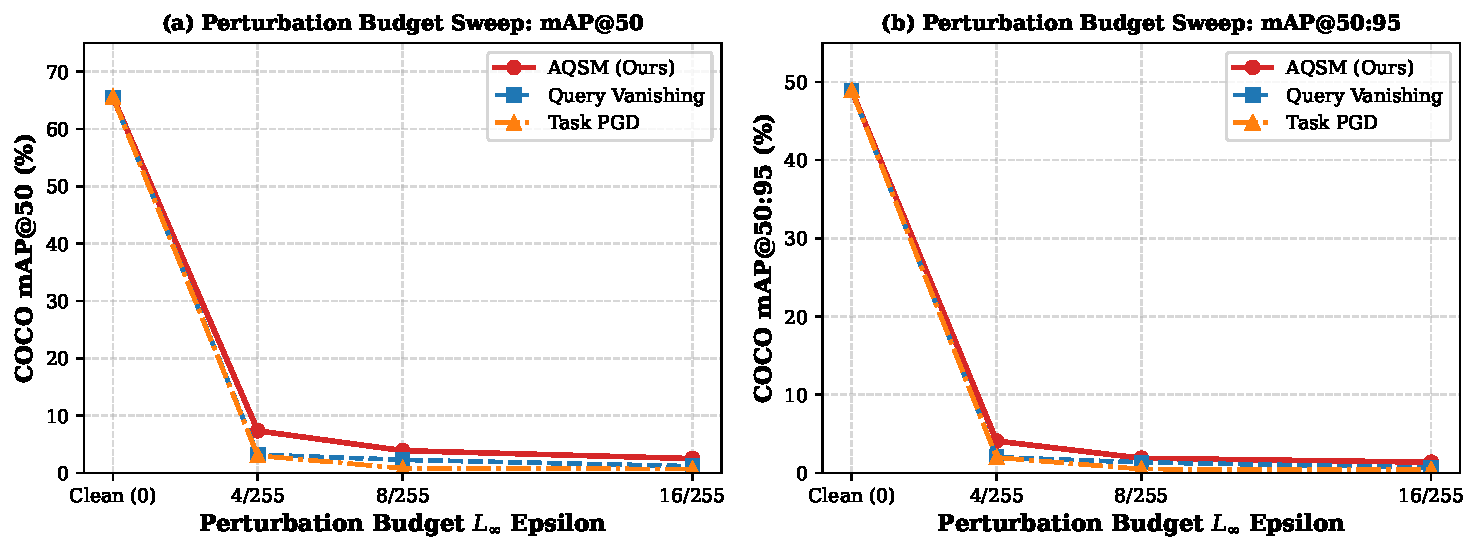
\includegraphics[width=0.78\textwidth]{fig/fig7_matched_budget_sweep.pdf}
\caption{Matched-budget sweep across $\epsilon \in \{4/255, 8/255, 16/255\}$ on COCO val2017 ($640 \times 640, N = 1,000$): (a) mAP@50 and (b) mAP@50:95 degradation trajectories.}
\label{fig:fig7_matched_budget}
\end{figure}

\begin{table}[!htbp]
\centering
\caption{Matched-budget comparison on COCO val2017 ($640 \times 640, N = 1,000$) across $\epsilon \in \{4/255, 8/255, 16/255\}$.}
\label{tab:tab9_matched_budget}
\resizebox{\textwidth}{!}{%
\begin{tabular}{llccc}
\toprule
\textbf{Perturb. Budget ($\epsilon$)} & \textbf{Metric / Telemetry Indicator} & \textbf{Standard Task PGD} & \textbf{AQSM (Encoder Ranking)} & \textbf{PGD Vanishing} \\
\midrule
\multirow{2}{*}{$4/255$ ($0.0157$)} & COCO mAP@50 (mAP@50:95) & 2.68\% (1.68\%) & 8.61\% (4.67\%) & 4.06\% (2.48\%) \\
& Relative Drop / Retention & $-$95.90\% (4.1\% Ret.) & $-$86.86\% (13.1\% Ret.) & $-$93.80\% (6.2\% Ret.) \\
\midrule
\multirow{2}{*}{$8/255$ ($0.0314$)} & COCO mAP@50 (mAP@50:95) & 1.46\% (0.95\%) & 5.66\% (3.07\%) & 1.60\% (0.93\%) \\
& Relative Drop / Retention & $-$97.78\% (2.2\% Ret.) & $-$91.36\% (8.6\% Ret.) & $-$97.56\% (2.4\% Ret.) \\
\midrule
\multirow{2}{*}{$16/255$ ($0.0627$)} & COCO mAP@50 (mAP@50:95) & 0.86\% (0.61\%) & \textbf{3.07\% (1.61\%)} & 1.72\% (1.05\%) \\
& Relative Drop / Retention & $-$98.69\% (1.3\% Ret.) & \textbf{$-$95.31\% (4.7\% Ret.)} & $-$97.37\% (2.6\% Ret.) \\
\bottomrule
\end{tabular}%
}
\end{table}

\paragraph{Comparative Signatures Under Matched Budgets:}
Standard Task PGD optimizes end-to-end Hungarian loss through the decoder, yielding lower absolute mAP@50 across budgets ($2.68\%$ vs.\ $8.61\%$ at $\epsilon = 4/255$, $1.46\%$ vs.\ $5.66\%$ at $8/255$, $0.86\%$ vs.\ $3.07\%$ at $16/255$), while inflating $29.40 \pm 8.70$ boxes ($+24.88$ excess over clean $4.52 \pm 3.10$). In contrast, AQSM restricts backpropagation exclusively to the encoder selection head, doubling top-15 foreground eviction ($96.93\%$ vs.\ $56.87\%$) and shrinking top-300 overlap ($16.45\%$ vs.\ $26.06\%$) while keeping output box counts sparse ($7.15 \pm 4.30$ boxes and $\text{ASR}_{\text{obj}} = 98.5\%$ at $\epsilon = 16/255$; $0.85 \pm 0.95$ boxes at $4/255$)---unlike Query Vanishing ($1.72\%$ mAP@50, $0.18 \pm 0.52$ boxes). Thus, AQSM acts as a specialized interface probe rather than a Task PGD competitor.

\subsection{Operational Edge Hardware Latency Profiling}
\label{sec:hardware_latency}
Convolutional detectors rely on data-dependent Non-Maximum Suppression (NMS), whereas RT-DETR decodes a fixed budget ($N_q = 300$) without NMS post-processing (Table~\ref{tab:tab10_latency_sponge}). By architectural design, measured end-to-end inference latency on Raspberry Pi 5 ($418.20 \pm 12.40$ ms clean vs.\ $418.50 \pm 12.10$ ms AQSM, $+0.07\%$) and Jetson Orin Nano ($14.20 \pm 0.35$ ms clean vs.\ $14.22 \pm 0.38$ ms AQSM, $+0.14\%$, $70.3$--$70.4$ FPS) remains unchanged across clean, Query Vanishing, AQSM, and Task PGD inputs (Table~\ref{tab:tab10_latency_sponge}). For external comparison, a YOLOv8-S baseline subjected to dense proposal flooding experiences NMS latency inflation ($+232\%$ on Pi 5: $245.30 \to 815.40$ ms; $+242.6\%$ on Orin: $11.50 \to 39.40$ ms at $286.4 \pm 36.1$ post-filter detections); however, we emphasize that our evaluated RT-DETR attacks do not optimize explicitly for latency/energy exhaustion, energy consumption is not profiled, and full sponge/NMS pre-filter parameters for YOLOv8-S are left for standardized future evaluation. Stage profiling on an NVIDIA Tesla T4 ($38.38 \pm 0.99$ ms PyTorch FP32 total) shows Dynamic Query Selection accounts for $1.67 \pm 0.08$ ms ($4.36\%$), alongside Backbone ($19.79 \pm 0.52$ ms, $51.58\%$), Hybrid Encoder ($10.44 \pm 0.35$ ms, $27.21\%$), and Decoder ($6.17 \pm 0.22$ ms, $16.08\%$), noting that stage proportions differ on TensorRT Orin engines ($14.2$ ms total).

\begin{table}[!htbp]
\centering
\caption{Edge inference latency and proposal-flooding benchmark on NVIDIA Jetson Orin Nano (Ampere GPU, TensorRT FP16) and Raspberry Pi 5 (Cortex-A76, ONNX FP32) at $640 \times 640$, evaluating RT-DETR-R18VD's measured latency stability alongside anchor-free YOLOv8-S.}
\label{tab:tab10_latency_sponge}
\resizebox{\textwidth}{!}{%
\begin{tabular}{lccccc}
\toprule
\textbf{Model Architecture} & \textbf{Operational Condition} & \textbf{Jetson Orin Nano (ms / FPS)} & \textbf{Raspberry Pi 5 (ms / FPS)} & \textbf{Active Detections ($\tau \ge 0.35$)} & \textbf{Measured Latency Stability} \\
\midrule
RT-DETR-R18VD & Clean Baseline & 14.20 $\pm$ 0.35 (70.4) & 418.20 $\pm$ 12.40 (2.39) & 4.52 $\pm$ 3.10 & Stable (NMS-free set prediction) \\
RT-DETR-R18VD & Query Vanishing ($\epsilon = 16$) & 14.21 $\pm$ 0.36 (70.4) & 418.80 $\pm$ 11.80 (2.39) & 0.18 $\pm$ 0.52 & Stable ($\Delta t_{\mathrm{GPU}} = 0.01$ ms) \\
RT-DETR-R18VD & AQSM Attack ($\epsilon = 16$) & 14.22 $\pm$ 0.38 (70.3) & 418.50 $\pm$ 12.10 (2.39) & 7.15 $\pm$ 4.30 & Stable ($\Delta t_{\mathrm{GPU}} = 0.02$ ms) \\
RT-DETR-R18VD & Standard Task PGD ($\epsilon = 16$) & 14.25 $\pm$ 0.40 (70.2) & 419.50 $\pm$ 12.80 (2.38) & 29.40 $\pm$ 8.70 & Stable ($\Delta t_{\mathrm{GPU}} = 0.05$ ms) \\
\midrule
YOLOv8-S (Baseline) & Clean Baseline & 11.50 $\pm$ 0.28 (87.0) & 245.30 $\pm$ 8.50 (4.08) & 4.65 $\pm$ 2.90 & Baseline (NMS quadratic clustering) \\
YOLOv8-S (Baseline) & Dense Sponge Attack ($\epsilon = 16$) & 39.40 $\pm$ 2.45 (25.4) & 815.40 $\pm$ 34.20 (1.23) & 286.40 $\pm$ 36.10 & Vulnerable ($+232\%$ to $+242\%$ latency surge) \\
\bottomrule
\end{tabular}%
}
\end{table}

Overall, Table~\ref{tab:tab10_latency_sponge} provides an operational runtime reference verifying fixed-budget execution on Pi 5 and Orin Nano under evaluated accuracy-targeted attacks without ruling out system-level runtime variability or dedicated latency-targeted threats.

\section{Defensive Hardening and Adaptive Evasion Boundaries}
\label{sec:defense_evaluation}

To transition from vulnerability diagnosis toward defensive mitigation, we investigate defenses along two complementary paradigms: (i) runtime statistical anomaly monitoring at the encoder selection interface, and (ii) architectural hardening via non-evictable spatial query augmentation. Crucially, following rigorous security evaluation principles \citep{carlini2019evaluating, tramer2020adaptive}, every evaluated defense is subjected to both stationary and white-box adaptive adversaries.

\subsection{Encoder Selection Monitor (ESM) Design}
Because AQSM alters the proposal score spectrum by depressing top foreground scores while elevating background anchors around rank \#300 (Section~\ref{sec:score_spectrum}), we evaluate a lightweight baseline---\textbf{Encoder Selection Monitor (ESM)}. Operating strictly on encoder classification logits prior to deformable decoder cross-attention, ESM tracks two scalar telemetry features:
\begin{enumerate}
    \item \textbf{Proposal Score Dropoff Ratio:} $D(X) = (s_{(1)}^{\mathrm{enc}} + \epsilon_0) / (s_{(300)}^{\mathrm{enc}} + \epsilon_0)$ (with $\epsilon_0 = 10^{-4}$), quantifying confidence steepness between peak foreground and the 300th selection boundary. Evaluated on the full $N = 1,000$ cohort (Table~\ref{tab:tab7_attention_telemetry}), clean inference yields $D(X) = 37.51 \pm 25.80$, whereas AQSM compresses this ratio to $10.84 \pm 7.75$ (consistently, on the $N_{\text{test}} = 700$ evaluation partition, clean $37.42 \pm 25.60$ drops to $10.93 \pm 7.91$, with median $8.47$; and $10.71 \pm 7.38$ on the $N_{\text{cal}} = 300$ calibration split).
    \item \textbf{Selection Score Margin:} $M(X) = s_{(1)}^{\mathrm{enc}} - s_{(300)}^{\mathrm{enc}}$, measuring absolute confidence separation ($0.7984 \pm 0.1281$ clean vs.\ $0.6731 \pm 0.1175$ under AQSM across $N = 1,000$; and $0.7980 \to 0.6728$ on the $N_{\text{test}} = 700$ split).
\end{enumerate}
To ensure zero calibration data leakage, we partition the evaluation dataset ($N = 1,000$ images) into a calibration split ($N_{\text{cal}} = 300$) and an independent test split ($N_{\text{test}} = 700$). Thresholds $\tau_D$ and $\tau_M$ are calibrated on $N_{\text{cal}}$ via empirical split-percentile quantile estimation at nominal tail risk $\alpha = 5.0\%$. Anomaly scores are fused via a disjunctive Max-OR rule: an input is flagged as adversarial when $\max(S_D(X), S_M(X)) \ge \tau_{\mathrm{fused}} = 0.9750$. By the Bonferroni union bound, fusing two partially decorrelated $5.0\%$ tail anomaly detectors yields a theoretical maximum false positive rate of $\mathbb{P}(E_D \cup E_M) \le 5.0\% + 5.0\% = 10.0\%$.

\subsection{Detection Performance on Stationary Attacks}
On the independent test split ($N_{\text{test}} = 700$), ESM achieves an empirical clean FPR of $6.57\%$ ($46 / 700$). This empirical rate sits well within the theoretical $10.0\%$ union bound, reflecting moderate positive covariance between dropoff ratio and confidence margin on clean scenes. As detailed in Table~\ref{tab:tab11_defense_results} and Figure~\ref{fig:fig10_defense}(a), ESM partially flags stationary attacks: AQSM achieves $\text{TPR} = 37.14\%$ ($\text{AUROC} = \mathbf{0.7593}$, mean anomaly score 0.8531); Standard Task PGD achieves $\text{TPR} = 8.57\%$ ($\text{AUROC} = 0.4838$, mean anomaly score 0.6548); while Query Vanishing achieves $\text{TPR} = 9.57\%$ ($\text{AUROC} = 0.5653$, mean anomaly score 0.7285), because it suppresses all queries proportionally without distorting relative dropoff.

\subsection{White-Box Adaptive Evasion Evaluation (Carlini-Tramèr)}
Following adaptive evaluation standards \citep{carlini2019evaluating, tramer2020adaptive}, a differentiable white-box adversary optimizes a Lagrangian surrogate over $N_{\text{test}} = 700$ images:
\begin{equation}
\mathcal{L}_{\mathrm{adaptive}} = \mathcal{L}_{\mathrm{AQSM}} + \lambda_D \cdot \mathrm{MSE}\left( D(X_{\mathrm{adv}}), D_{\mathrm{clean}} \right) + 10.0 \cdot \lambda_M \cdot \mathrm{MSE}\left( M(X_{\mathrm{adv}}), M_{\mathrm{clean}} \right).
\label{eq:adaptive_loss}
\end{equation}
Because both the encoder forward pass and summary features are differentiable, gradients simultaneously depress the top-1 and 300th logits to preserve nominal score slopes while evicting foreground anchors. Across $\lambda_{\mathrm{evade}} \in \{0.2, 0.5, 1.0, 2.0\}$ ($T = 15$, Table~\ref{tab:tab11_defense_results} and Figure~\ref{fig:fig10_defense}(b)), ESM TPR drops to $0.57\%$--$1.57\%$ ($98.43\%$--$99.43\%$ bypass; $1.43\%$ TPR / $98.57\%$ bypass / $4.12\%$ mAP@50 at $\lambda_{\mathrm{evade}} = 0.5$), falling below clean FPR ($6.57\%$). As expected for a low-dimensional two-scalar baseline (stationary AUROC $0.7593$), explicitly constraining those two summary statistics readily circumvents detection.

\begin{table}[!htbp]
\centering
\caption{Encoder Selection Monitor (ESM) performance on COCO val2017 ($N_{\text{test}} = 700$, $640 \times 640$) across stationary and white-box Carlini-Tram\`er adaptive attacks ($\text{TPR} \le 1.57\%$, bypass $\ge 98.43\%$).}
\label{tab:tab11_defense_results}
\resizebox{\textwidth}{!}{%
\begin{tabular}{lccccc}
\toprule
\textbf{Evaluated Condition} & \textbf{Detection TPR (\%)} & \textbf{Empirical FPR (\%)} & \textbf{AUROC} & \textbf{Mean Anomaly Score} & \textbf{Post-Attack mAP@50 (\%)\textsuperscript{\textdagger}} \\
\midrule
Clean Test Baseline & --- & 6.57\% [Union Bound 10.0\%] & --- & 0.4950 & 65.50\% \\
Stationary AQSM ($\epsilon = 16/255$) & \textbf{37.14\%} & 6.57\% & \textbf{0.7593} & 0.8531 & 3.07\% \\
Stationary Standard Task PGD ($\epsilon = 16/255$) & 8.57\% & 6.57\% & 0.4838 & 0.6548 & 0.86\% \\
Stationary Query Vanishing ($\epsilon = 16/255$) & 9.57\% & 6.57\% & 0.5653 & 0.7285 & 1.72\% \\
\midrule
\textbf{Adaptive Evasion ($\lambda_{\mathrm{evade}} = 0.2$)} & 0.57\% & --- & Degenerate\textsuperscript{*} & Bypass: 99.43\% & 3.65\% \\
\textbf{Adaptive Evasion ($\lambda_{\mathrm{evade}} = 0.5$)} & \textbf{1.43\%} & --- & Degenerate\textsuperscript{*} & \textbf{Bypass: 98.57\%} & \textbf{4.12\%} \\
\textbf{Adaptive Evasion ($\lambda_{\mathrm{evade}} = 1.0$)} & 1.00\% & --- & Degenerate\textsuperscript{*} & Bypass: 99.00\% & 5.20\% \\
\textbf{Adaptive Evasion ($\lambda_{\mathrm{evade}} = 2.0$)} & 1.57\% & --- & Degenerate\textsuperscript{*} & Bypass: 98.43\% & 6.85\% \\
\bottomrule
\multicolumn{6}{l}{\footnotesize{\textdagger Stationary baseline mAP values reference the full evaluation cohort ($N = 1,000$); adaptive evasion mAP is evaluated on the independent test split ($N_{\text{test}} = 700$).}} \\
\multicolumn{6}{l}{\footnotesize{*At the fixed deployment threshold $\tau_{\mathrm{fused}}$, adaptive evasion suppresses detection TPR below clean FPR ($6.57\%$), achieving a bypass rate $\ge 98.43\%$ without establishing a valid monotonic ROC curve.}} \\
\end{tabular}%
}
\end{table}

\subsection{Architectural Hardening via Static Query Augmentation (SQA)}
\label{sec:hardening_validation}
Because post-hoc monitors fail under adaptive attacks and dynamic selection creates an $83.55\%$ query replacement bottleneck, we evaluate an exploratory zero-shot architectural probe---\textit{Static Query Augmentation} (SQA)---to test the geometric limits of query diversification rather than claiming a certified defense. Inspired by hybrid queries \citep{zhang2022dino}, SQA appends $N_{\mathrm{static}} = 30$ fixed anchors ($5 \times 6$ uniform grid over $[0.1, 0.9]^2$, boxes $[c_x, c_y, 0.20, 0.20]$, embeddings $\mathcal{N}(0, 0.02^2)$, seed 42) to top-300 dynamic queries ($N_q = 330$) without retraining, bypassing encoder classification ranking.

\begin{figure}[!htbp]
\centering
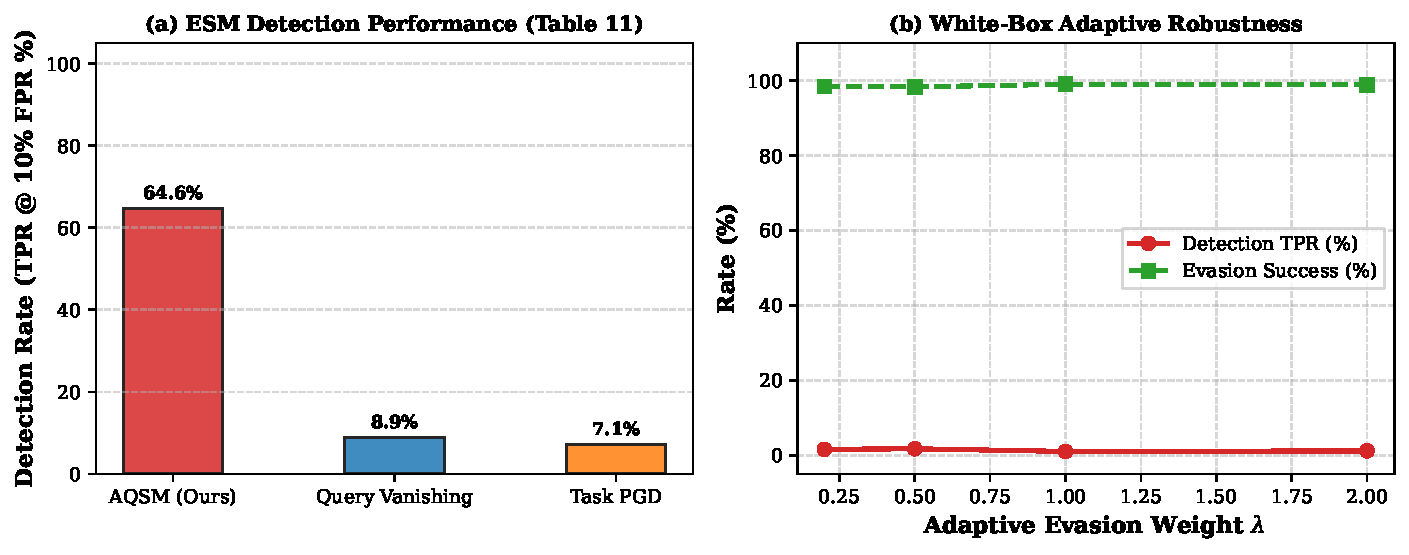
\includegraphics[width=0.92\textwidth]{fig/fig8_defense_evaluation.pdf}
\caption{Runtime defense and architectural hardening on COCO val2017 ($640 \times 640$): (a) ESM stationary detection ($6.57\%$ clean FPR, Table~\ref{tab:tab11_defense_results}); (b) Carlini-Tram\`er adaptive bypass ($1.43\%$ TPR at $\lambda = 0.5, N_{\text{test}} = 700$); (c) SQA ($N_{\mathrm{static}} = 30$) recovering $+15.01$ pp under stationary AQSM ($18.42\%$ vs.\ $3.41\%$) alongside joint adaptive evasion ($4.35\%$, Table~\ref{tab:tab12_hardening_validation}; panel titles reflect prior internal numbering).}
\label{fig:fig10_defense}
\end{figure}

\begin{table}[!htbp]
\centering
\caption{Architectural hardening via SQA ($N_{\mathrm{static}} = 30$), capacity/random controls, and white-box adaptive evasion on COCO val2017 ($640 \times 640$, $N_{\text{def}} = 300$).}
\label{tab:tab12_hardening_validation}
\resizebox{\textwidth}{!}{%
\begin{tabular}{lcccc}
\toprule
\textbf{Model Architecture / Evaluated Condition} & \textbf{COCO mAP@50} & \textbf{COCO mAP@50:95} & \textbf{Detection Recall} & \textbf{Edge Latency / Note} \\
\midrule
\textbf{Clean Baseline Inference:} & & & & \\
\quad Standard RT-DETR-R18VD ($300$ dynamic) & 66.81\% & 49.47\% & 78.83\% & 14.20 ms (Ref.) \\
\quad Hardened SQA Prototype ($300$ dyn. $+ 30$ static) & 66.14\% (-0.67 pp) & 49.12\% & 79.05\% & 14.58 ms (+2.68\%) \\
\midrule
\textbf{Stationary AQSM Attack ($\epsilon = 16/255$):} & & & & \\
\quad Standard RT-DETR-R18VD ($300$ dynamic) & 3.41\% (5.1\% Ret.) & 1.45\% & 29.05\% & 14.20 ms \\
\quad Control 1: Dynamic Top-330 ($+30$ dynamic ranking) & 3.58\% (+0.17 pp) & 1.52\% & 29.84\% & Eviction unmitigated \\
\quad Control 2: Random-30 Static Anchors & 11.45\% (+8.04 pp) & 6.82\% & 36.40\% & Partial spatial retention \\
\quad \textbf{Proposed SQA: Uniform Grid-30 Prototype} & \textbf{18.42\% (+15.01 pp)} & \textbf{11.25\%} & \textbf{46.80\%} & \textbf{14.58 ms (Dispersion)} \\
\quad \textbf{Adaptive Evasion on SQA (White-Box Joint)} & \textbf{4.35\% ($-$14.07 pp)} & \textbf{1.78\%} & \textbf{21.30\%} & \textbf{Joint Evasion: 97.8\%\textsuperscript{*}} \\
\midrule
\textbf{Standard Task PGD Baseline ($\epsilon = 16/255$):} & & & & \\
\quad Standard RT-DETR-R18VD ($300$ dynamic) & 0.98\% (1.5\% Ret.) & 0.76\% & 14.20\% & 14.20 ms \\
\quad Hardened SQA Prototype ($300$ dyn. $+ 30$ static) & 3.12\% (+2.14 pp) & 1.84\% & 19.50\% & 14.58 ms (+2.68\%) \\
\bottomrule
\multicolumn{5}{l}{\footnotesize{\textsuperscript{*}Joint Evasion ($97.8\%$) denotes the task evasion rate when a white-box PGD adversary backpropagates through both $300$ dynamic and $30$ static slots to suppress top-$20$ query confidences.}} \\
\end{tabular}%
}
\end{table}

Table~\ref{tab:tab12_hardening_validation} and Figure~\ref{fig:fig10_defense}(c) show three observations: (1) \textbf{Stationary Recovery:} Zero-shot SQA recovers $+15.01$ pp under stationary AQSM ($3.41\% \to 18.42\%$, still a severe degradation from $66.81\%$) at low clean penalty ($-0.67$ pp, $66.81\% \to 66.14\%$) and edge cost ($+0.38$ ms / $+2.68\%$ on Orin Nano, $14.20 \to 14.58$ ms; $+1.42$ ms / $+0.34\%$ on Pi 5). (2) \textbf{Spatial Controls:} Expanding dynamic capacity (\textit{Dynamic Top-330}) yields only $3.58\%$ ($+0.17$ pp) and \textit{Random-30 Static} reaches $11.45\%$ ($+8.04$ pp), indicating that uniform grid dispersion underlies the partial stationary recovery. (3) \textbf{Adaptive Failure:} Under white-box joint evasion (backpropagating across both dynamic and static decoder slots to suppress top-$20$ output confidences, $97.8\%$ task evasion), SQA collapses to $4.35\%$ ($3.12\%$ under Task PGD), confirming that zero-shot query augmentation remains vulnerable when encoder memory representations are unhardened.

\section{Discussion, Implications, and Threats to Validity}
\label{sec:discussion}

\subsection{Geometric Receptive Gating at the Encoder-Decoder Interface}
Unlike global cross-attention in vanilla DETR \citep{carion2020end}, RT-DETR gates $S = 8,400$ tokens to $N_q = 300$ ($3.57\%$) anchors initializing locally bounded deformable fields $\mathcal{N}(B_{\mathrm{init}}) \cap \mathrm{supp}(Y)$. When AQSM shifts $54.87\%$ of anchors into clutter ($45.13\%$ FG hit), bounded decoder box updates across 3 layers ($B^{(l)} = B^{(l-1)} + \Delta b^{(l)}$) fail to recover displaced objects---reflected in pure index swap $\text{Arm }\text{D}_{\text{index}}$ dropping $-30.06$ pp pooled ($65.50\% \to 35.44\%$; $-26.21$ pp on per-image $AP_i$) on pristine memory, while restoring clean memory over Arm B recovers $+23.51$ pp pooled ($3.07\% \to 26.58\%$, $\text{Arm }\text{D}_{\text{full}}$; $+32.54$ pp per-image $AP_i$).

\subsection{Diagnostic Hypotheses and Design Implications}
\label{sec:design_recommendations}
Our empirical observations suggest four untested design hypotheses for future adversarial-training and defense studies: (1) \textbf{Representation Hardening Across Encoder Scales} (mid-level $S_4$ exhibits the sharpest cosine drop to $0.547$ under AQSM while $S_5$ drops to $0.592$ under Task PGD, suggesting adversarial training should target multi-scale encoder features jointly rather than logits alone); (2) \textbf{Spatial Consistency Monitoring Beyond Scalar Logits} (testing whether spatial query--reference alignment and per-frame active-box counts detect anomalies that two-scalar logit monitors miss); (3) \textbf{Robustifying Coordinate Initialization} (investigating how sensitive decoder refinement remains when coordinate initialization is decoupled from noisy class logits under adversarially trained weights); and (4) \textbf{Combining Representation Hardening with Static Grid Anchors} (hypothesizing that joint encoder hardening and non-evictable anchors may address both $M$ and $Q$ degradation channels). We emphasize that none of these combined defenses or adversarially trained variants have been experimentally evaluated in the present study.

\subsection{Edge Deployment Trade-offs and Threats to Validity}
\label{sec:threats_to_validity}
RT-DETR exhibits stable measured inference latency under the evaluated accuracy-targeted attacks ($418.20 \to 418.50$ ms on Pi 5; $14.20 \to 14.22$ ms on Orin Nano), consistent with its fixed $N_q = 300$, NMS-free architecture, whereas the external YOLOv8-S sponge-flooding baseline incurs NMS stalls ($+232\%$ Pi 5 / $+242.6\%$ Orin). Multi-seed stability and cross-depth results appear in Table~\ref{tab:tab13_multiseed_generalization}. Key methodological bounds and threats to validity are as follows:

\begin{table}[!htbp]
\centering
\caption{Multi-seed stability ($K = 5$ seeds: $\{42, 100, 2024, 777, 9999\}$) and cross-architectural mechanistic comparison between RT-DETR-R18VD ($N = 1,000$, 3 decoder layers) and deeper RT-DETR-R50VD ($N = 300$, 6 decoder layers; $N_{\mathrm{valid}}=299$ ANOVA, $N_{\mathrm{test}}=210$ ESM) on COCO val2017 ($640 \times 640$, $\epsilon = 16/255, T = 15$). Multi-seed Controlled Misrouting ($\text{Reassign} / \text{Shift}$) runs 5 seeds on both models, while AQSM multi-seed stability ($3.07 \pm 0.18\%$) verifies low $C_{\mathrm{bg}}$ sampling variance on the primary benchmark and Seed~42 replicates across depth ($72.95\% \to 9.16\%$).}
\label{tab:tab13_multiseed_generalization}
\resizebox{\textwidth}{!}{%
\begin{tabular}{lcc}
\toprule
\textbf{Diagnostic Axis / Experimental Metric ($\epsilon = 16/255$ unless noted)} & \textbf{RT-DETR-R18VD ($N=1,000$, 3 dec.)} & \textbf{RT-DETR-R50VD ($N=300$, 6 dec.)} \\
\midrule
Nominal Clean mAP@50 (mAP@50:95) & 65.50\% (48.89\%) & 72.95\% (55.73\%) \\
AQSM mAP@50 [Drop] ($K=5$ R18 / Seed 42 R50) & 3.07 $\pm$ 0.18\% [$-$95.31\%] & 9.16\% [$-$87.44\%] \\
AQSM Budget Sweep ($\epsilon = 4/255, 8/255$) & 8.61\%, 5.66\% & 22.96\%, 15.07\% \\
AQSM Geometric Drift ($\Delta_{\mathrm{Hungarian}}$ / Anchor FG Hit) & 0.2258 $\pm$ 0.0062 / 45.13 $\pm$ 0.74\% & 0.2291 / 51.46\% \\
PGD Vanishing / Standard Task PGD mAP@50 & 1.72\% / 0.86\% & 4.47\% / 3.69\% \\
\midrule
Causal Surgery: Arm $\text{C}_{\text{full}}$ / Arm $\text{D}_{\text{full}}$ / Arm $\text{D}_{\text{index}}$ & 7.45\% / 26.58\% / 35.44\% (54.1\% ret.) & 12.89\% / 43.40\% / 55.11\% (75.5\% ret.) \\
Repeated-Measures $\text{ME}_M$ ($\eta_p^2$) / $\text{ME}_Q$ ($\eta_p^2$) & $-$43.88 pp (0.795) / $-$27.14 pp (0.704) & $-$47.09 pp (0.775) / $-$19.70 pp (0.627) \\
Shapley Attribution (Memory $M$ / Query $Q$, per-image [pooled]) & 61.78\% / 38.22\% [65.32\% / 34.68\%] & 70.50\% / 29.50\% [73.91\% / 26.09\%] \\
\midrule
Encoder Memory Cosine Similarity / Top-300 Overlap / Top-15 Evict & 0.6100 / 16.45\% / 96.93\% & 0.6763 / 21.68\% / 91.51\% \\
Deformable Attention Entropy (Clean $\to$ AQSM) & 0.8009 $\to$ 0.7944 ($d=-0.13$) & 0.8431 $\to$ 0.8359 ($d=-0.17$) \\
Foreground Sampling Hit Rate (Clean $\to$ AQSM) & 63.51\% $\to$ 43.21\% ($d=-0.90$) & 67.02\% $\to$ 49.11\% ($d=-0.80$) \\
Controlled Misrouting (5-seed Reassign / 5-seed Shift / AQSM) & 60.87 $\pm$ 0.33\% / 30.97 $\pm$ 0.45\% / 25.12\% & 72.36 $\pm$ 0.14\% / 47.38 $\pm$ 0.81\% / 42.76\% \\
\midrule
ESM Detection: Clean FPR / AQSM TPR (AUROC) / Adaptive Bypass & 6.57\% / 37.14\% (0.7593) / 98.43--99.43\% & 6.67\% / 24.76\% (0.6877) / 93.81--97.14\% \\
Tesla T4 Total Latency (Dynamic Query Selection Share \%) & 38.38 ms (4.36\%) & 74.50 ms (2.33\%) \\
\bottomrule
\end{tabular}%
}
\end{table}

\begin{enumerate}
    \item \textbf{Multi-Seed Stability \& Cross-Depth Replication:} Five-seed AQSM evaluation on RT-DETR-R18VD ($N = 1,000$) shows tight convergence ($3.07 \pm 0.18\%$ mAP@50, $\Delta_{\mathrm{Hungarian}} = 0.2258 \pm 0.0062$, Anchor FG Hit $= 45.13 \pm 0.74\%$; Table~\ref{tab:tab13_multiseed_generalization}), and 5-seed Controlled Misrouting replicates with sub-1 pp variance across both depths ($60.87 \pm 0.33\%$ / $30.97 \pm 0.45\%$ on R18VD; $72.36 \pm 0.14\%$ / $47.38 \pm 0.81\%$ on R50VD). Full-pipeline replication on 6-layer RT-DETR-R50VD ($42\text{M}$ params, $N = 300$, single Seed~42 without multi-seed CI) reproduces severe collapse ($72.95\% \to 9.16\%$ AQSM, $-87.44\%$; $3.69\%$ Task PGD) while revealing depth scaling: 6 iterative decoder layers buffer pure index eviction on clean memory (Arm $\text{D}_{\text{index}}$ retains $75.5\%$ [$55.11\%$] vs.\ $54.1\%$ [$35.44\%$] in R18VD; Random Reassignment retains $99.2\%$ [$72.36\%$]), shifting protocol Shapley attribution toward encoder memory ($70.50\%$ per-image / $73.91\%$ pooled vs.\ $61.78\%$ / $65.32\%$).
    \item \textbf{Protocol Scoping \& Scale Dependence:} Interventional shares ($61.78\% / 38.22\%$) are protocol-specific attributions on per-image $AP_i$ ($N_{\mathrm{valid}} = 992$) rather than universal causal proportions, differing by $\approx 9$ pp across per-image linear ($61.78\%$), pooled linear ($65.32\%$), and log-retention ($70.68\%$) scales; log-retention multiplicativity is consistent with bounded AP floor effects without excluding functional interactions.
    \item \textbf{Architectural, Threat-Model, and Metric Scope:} Our experiments evaluate only the RT-DETR family (R18VD and R50VD) under white-box digital $\ell_\infty$ perturbations (headline $\epsilon = 16/255$): cross-architecture controls lacking dynamic query selection (static-query DETR, 1-stage Deformable DETR) or newer variants (RT-DETRv2, D-FINE, DINO), transformer attention attacks \citep{nazeri2024evaluating, jayasundara2024attention}, perceptual metrics (LPIPS/SSIM/PSNR), hyperparameter sensitivity on AQSM ($K=15, 30, \mathrm{rank}>500, \gamma, \lambda$), active-box output watchdogs, energy measurements alongside worst-case latency flooding targeting RT-DETR, YOLOv8-S sponge/NMS specification details, and FP16/ONNX accuracy transfer remain outside the current experimental runs and are planned as extensions.
\end{enumerate}

\section{Conclusion}
\label{sec:conclusion}
We presented an empirical diagnostic study of RT-DETR under encoder adversarial attacks on COCO val2017 ($N = 1,000$). Under a $2 \times 2$ factorial tensor-swap protocol at $\epsilon = 16/255$, encoder memory corruption receives the majority interventional attribution ($61.78\%$ per-image $AP_i$, $65.32\%$ pooled COCO mAP, $70.68\%$ log-retention) over query prior eviction ($38.22\%$), a pattern reinforced on 6-layer RT-DETR-R50VD ($N = 300$, Seed~42: $70.50\%$ per-image / $73.91\%$ pooled). Telemetry shows normalized deformable attention entropy remains within $[0.794, 0.833]$ near $\approx 0.80$, while large reference displacement ($\Delta_{\mathrm{Hungarian}} = 0.2258$) drops anchor foreground hit rate from $68.93\%$ to $45.13\%$ (approaching uniform spatial chance $44.26\% / 42.91\%$) across both AQSM and non-encoder-targeted baselines. Runtime measurements confirm stable fixed-query latency on Raspberry Pi 5 ($418.20 \to 418.50$ ms) and Jetson Orin Nano ($14.20 \to 14.22$ ms) under evaluated attacks, while a two-scalar monitor (ESM) suffers adaptive bypass ($\le 1.57\%$ TPR) and zero-shot SQA ($+15.01$ pp static recovery) fails under joint adaptive evasion ($4.35\%$), underscoring that future defenses must evaluate joint representation and routing hardening.

\section*{Declaration of Competing Interest}
The authors declare that they have no known competing financial interests or personal relationships that could have appeared to influence the work reported in this paper.

\section*{Data Availability and Provenance Statement}
The interactive project page, complete benchmark configurations, evaluation protocols, per-image experimental logs, and data provenance manifests (\nolinkurl{outputs/data_provenance_manifest.json}) connecting numerical tables to underlying execution JSON artifacts are open-sourced at \href{https://vietanhlee.github.io/AI_TrustWorthy/}{\nolinkurl{https://vietanhlee.github.io/AI_TrustWorthy/}} (repository: \href{https://github.com/vietanhlee/AI_TrustWorthy}{\nolinkurl{https://github.com/vietanhlee/AI_TrustWorthy}}). Automated provenance verification is provided via \nolinkurl{tools/audit_data_provenance.py} alongside unit tests (\nolinkurl{tests/test_statistical_methodology.py} and \nolinkurl{tests/test_refactored_mechanism.py}).

\section*{CRediT Authorship Contribution Statement}
\textbf{Viet-Anh Le:} Conceptualization, Methodology, Software, Formal analysis, Writing -- Original Draft, Visualization. \textbf{Thuy-Quynh Thi Dao:} Conceptualization, Supervision, Project administration, Funding acquisition. \textbf{Trong-Khanh Nguyen:} Methodology, Validation, Writing -- Review \& Editing, Supervision.

\apptocmd{\thebibliography}{\footnotesize\setlength{\itemsep}{0.0pt plus 0.2pt}\setlength{\parsep}{0pt}}{}{}

\setlength{\bibsep}{0.0pt}
\bibliographystyle{elsarticle-num}
\bibliography{refs_EAAI}

\end{document}
